
\section{Calibration and alignment}
\begin{figure*}
    \centering
    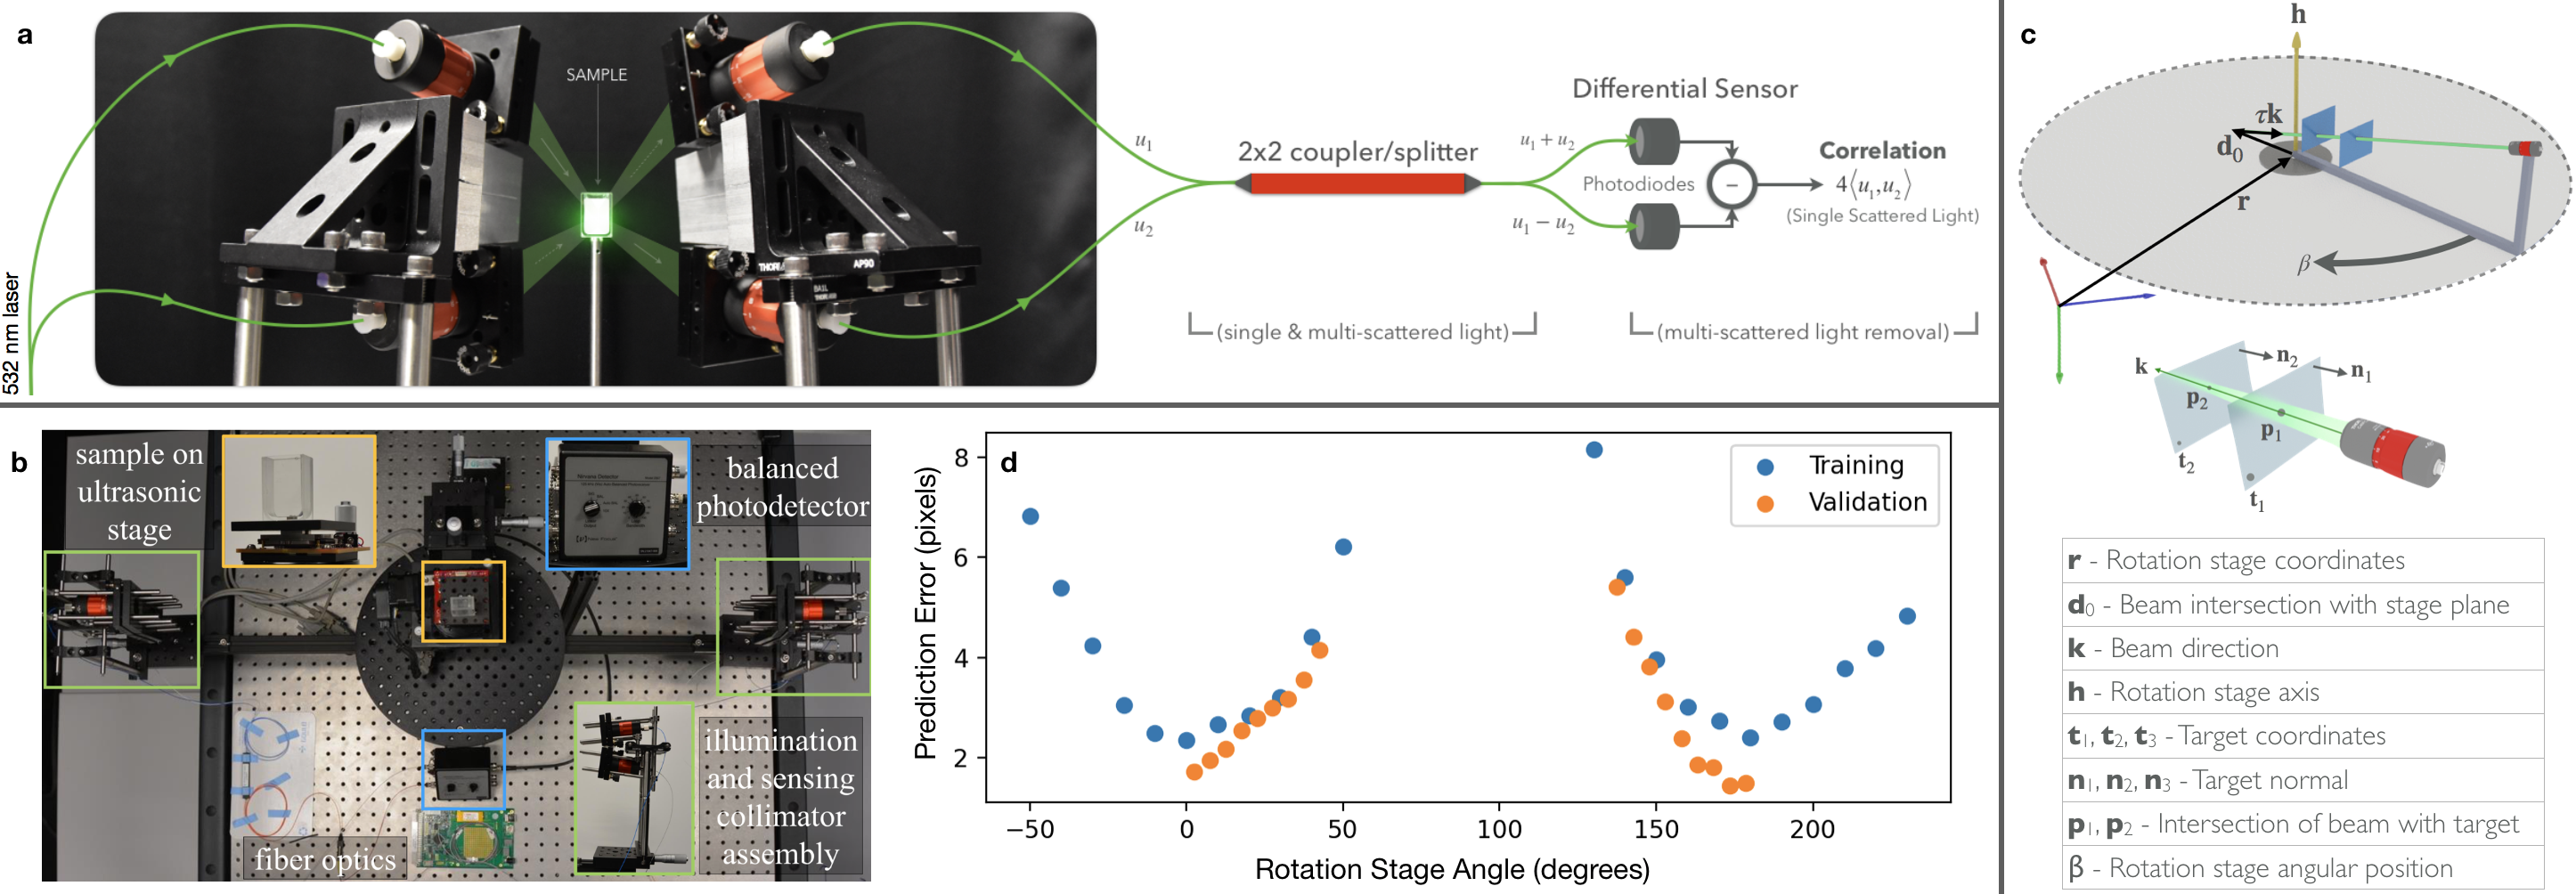
\includegraphics[width=\textwidth]{figures/experiment.png}
    \caption{\textbf{a}: Speckle correlation computation pipeline. The sample is illuminated by two beams, and the correlation is computed using a differential sensor. \textbf{b}: Physical setup with sample placed on the circular breadboard. The illumination stand rotates about the sample while the sensing stand measures scattered light. The differential photodetector enables fast correlation computation. \textbf{c}: Geometry used to develop forward model for inverse problem estimation of 3D beam-plane intersection points. \textbf{d}: Mean estimation errors for training and validation phases showing angular dependence of error.}
    \label{fig:3}
\end{figure*}

\section{Calibration Targets}
We use two primary checkerboard calibration targets for beam direction and pose estimation during scatterometer calibration and alignment. The first is a $12\times15$ checkerboard with 6.1mm spacing mounted on both faces of a $10\times10$cm Corning Gorilla Glass window. This target is used primarily for estimating rotation and translation stage axes and motion stage pose. The other primary target uses the same checkerboard size, but it is one-sided, and it is missing a $2\times9$ block of cherckerboard squares at its center. We explored many checkerboard sizes and found that squares sizes smaller than 5mm prouced noisy MATLAB camera calibration. We chose 6.1mm squares since it maximizes the checkerboard density while producing stable MATLAB camera calibration. Both targets are laser printed on standard office printer paper, so their actual sizes will differ from their intended sizes due to printer scaling, paper texture, and limited printing precision. One issue with the relatively small square size is that these printing errors become larger with respect to the square size, and errors of approximately 1\% can cause a depth error estimate of greater than 3mm. However, we were only able to measure their sizes to an accuracy of 3.5\%. We use a third $18\times25$ (7.5mm square size) calibration target that is UV printed on a rigid, low-density polyethylene board (LDPE) with 0.04mm precision as a reference. We determine the laser printed targets' square sizes in the following manner. We place all three targets at the same depth, and we estimate the reference target's depth assuming its nominal dimensions as ground truth. For each laser printed target, we find the square size that minimizes the difference between its depth and the reference target's depth. We verified our results by laser printing all targets on the same sheet of paper and confirming all three square size estimates were similar down to tens of microns. We detail the effects of albedo and square size analyses in Appendix \ref{appx:calibration_checkerboard_design}.

\section{Lower Stage Calibration} \label{sec:lower_stage_calibration}
The goal of calibrating the lower assembly is to estimate its rotation axis and the 3D orientation of the illumination beams as a function of the azimuth angle $\theta$. We do so by computing the 3D intersection of each illumination beam with a series of $N$ planes whose poses we know. This process is repeated for all $\theta \in \Theta$ for a total of $2N|\Theta|$ points. From this set of points, we can estimate the illumination directions for both beams as a function of $\theta$ and the azimuth stage pose up to a rotational ambiguity about its rotation axis.

\paragraph{Azimuth Stage Rotation Axis}
Each beam is associated with a set of $N|\Theta|$ points. Define a set of difference vectors $\{\tilde{\vec{k}}_\theta\}, \; |\{\tilde{\vec{k}}_\theta\}| = L$ as the differences between all N permute 2 points along a ray. We define a ray as a beam located at any particular $\theta \in \Theta$. Each $\tilde{\vec{k}}_\theta$ makes an angle $\pi/2 - \alpha$ with the rotation axis. However, the $_L P_2$ second order difference vectors are perpendicular to the azimuth rotation axis $\uvec{h}$, and we estimate $\uvec{h}$ as their null space.

\paragraph{Beam Direction for $\theta = 0$}
Once we know the azimuth rotation axis, we can use it to estimate both illuminators' beam directions. For each $\theta \in \Theta$, we compute the centroid $\vecol{p}_\theta = \frac{1}{N} \sum p_n$. We subtract the centroid from the point set so it is zero mean and rotate it about $\uvec{h}$ by $-\theta$ so all points are aligned with $\theta = 0$. The beam direction $\vec{k}_0$ is simply the point set's principal component.
%
\begin{figure}
    \centering
    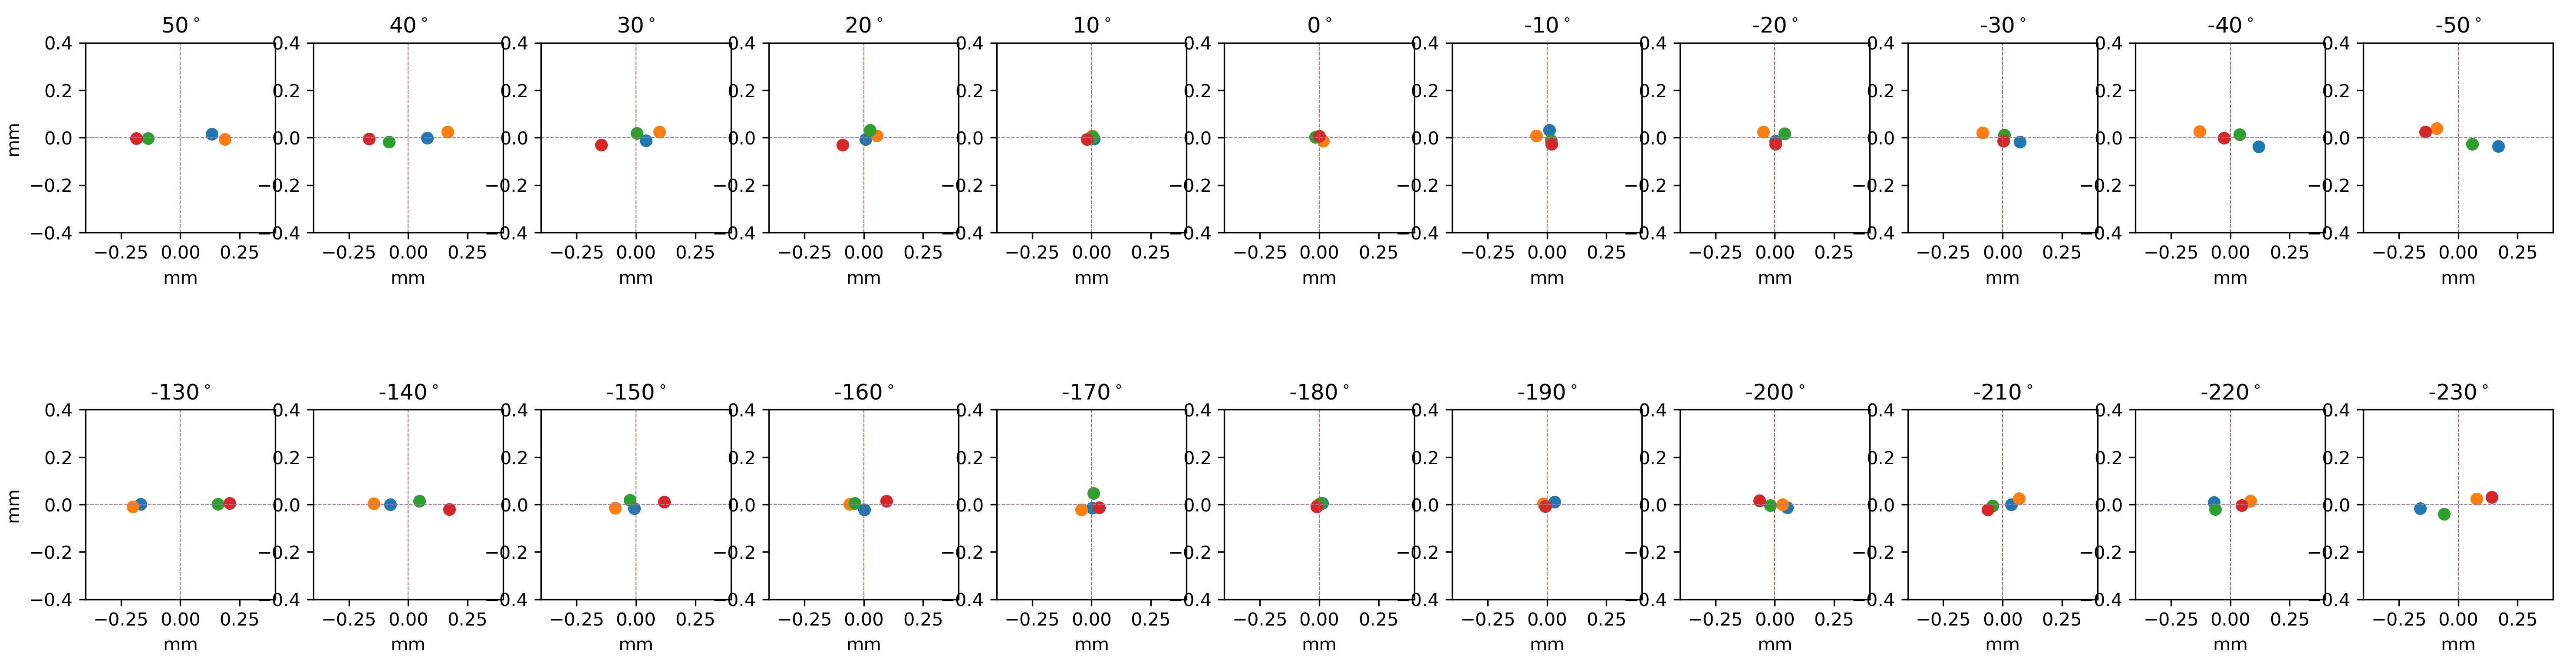
\includegraphics[width=1\linewidth]{figures/beam_direction_fits.png}
    \caption{Perpendicular offsets of the four observed beam-plane intersections with respect to the estimated beam direction. Each plot is for an azimuthal angle $\theta \in \Theta$. The cause of increasing perpendicular offsets for increasing angle with respect to the plane normal and anti-normal is unknown.}
    \label{fig:beam_direction_plane_points}
\end{figure}

\subsection{Stage Position \& Beam Direction as a Function of $\theta$}
Assume a collimated beam fixed to a rotation stage with location $\vec{r}$ and rotation axis $\uvec{h}$. If the stage is rotated 360 degrees, the pencil of rays created by the rotated beam will form a paraboloid with axis $\uvec{h}$ and small radius $\rho$ equal to the distance of closest encounter of the beam with the paraboloid axis. The locus of these points of closest encounter constitutes the beam's ray envelope. \note{Insert ray envelope theory} The isoline of the ray envelope is
%
\begin{figure}
    \centering
    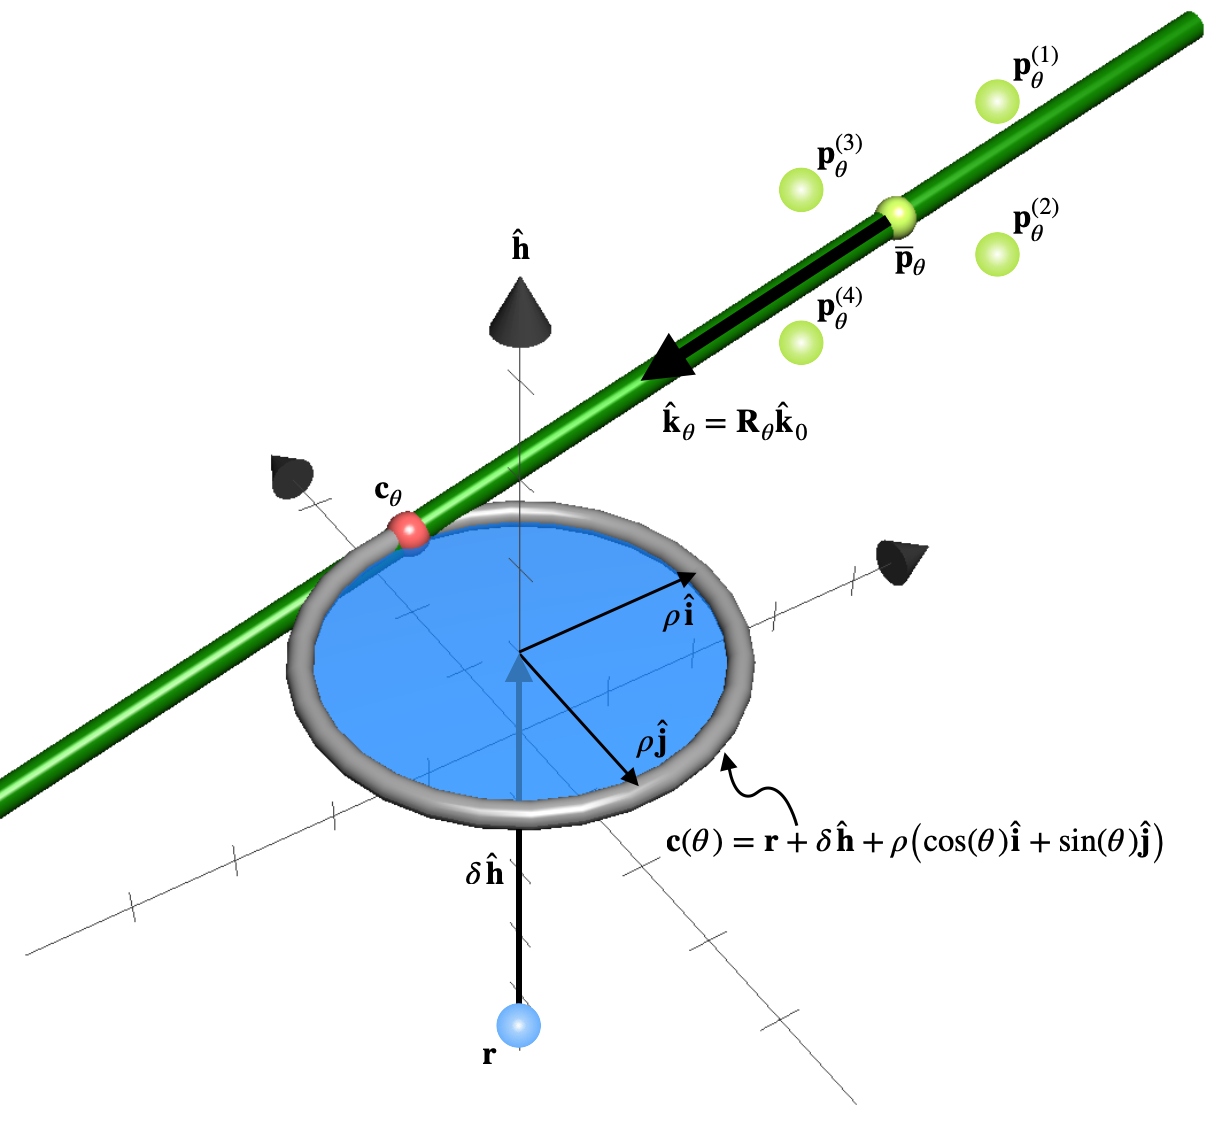
\includegraphics[width=0.5\linewidth]{figures/envelope_geometry.png}
    \caption{RT-5 Geometry - Frustrum top Surface}
    \label{fig:frustrum}
\end{figure}
%
\begin{equation}
    \vec{c}(\theta) = \vec{r} + \delta \uvec{h} + r(\theta) \vec{\rho}_0,
    \label{eqn:envelope}
\end{equation}
%
where $\delta$ is the height of the circle above the stage, $\vec{\rho}$ is a $2 \times 1$ vector. $r(\theta)$ is a $3 \times 2$ matrix consisting of a rotation of two basis vectors $\uvec{i}$ and $\uvec{j}$ through an angle of $\theta$ about the rotation axis $\uvec{h}$ with each basis vector being perpendicular to $\uvec{h}$
%
\begin{equation}
    r(\theta) = \vec{R}(\uvec{h}, \theta) \begin{bmatrix}
        \uvec{i} & \uvec{j}
    \end{bmatrix},
    \quad \vec{R}(\uvec{h}, \theta) \in \mathbb{R}^{3 \times 3}.
\end{equation}

If $M$ points $\vec{p}_\theta^{(1)}, \vec{p}_\theta^{(2)}, ..., \vec{p}_\theta^{(M)}$ are measured along the ray at a given rotation stage position $\theta \in \Theta$, then the beam with direction $\uvec{k}_{\theta}$ passes through their centroid $\vecol{p}_\theta$ with its pencil defined
%
\begin{align}
    \vec{l}_\theta(s) = \vecol{p}_\theta + s \uvec{k}_{\theta}
\end{align}

\subsection{Azimuth Stage Location}
Given the problem formulation, the objective is to find the circular conic section with perimeter $\vec{c}(\theta)$ by choosing $\vec{r}$ such that the circle's radius $\rho$ is minimized. We achieve this by computing the minimum distance of each beam from the axis of rotation and minimizing the variance across all angles:

\begin{align}
    \min_{\vec{r}} & \; g_2(\vec{r}) \\
    \min_{\vec{r}} & \; \sigma^2(\{\rho_\theta\}) \\
    \min_{\vec{r}} & \sum_{\theta \in \Theta} (\rho_\theta - \overline{\rho})^2
\end{align}
%
where
\begin{gather}
    \rho_\theta = \uvec{n}_\theta^\intercal (\vecol{p}_\theta - \vec{r}), \quad \uvec{n}_\theta = \frac{\uvec{k}_\theta \times \uvec{h}}{\| \uvec{k}_\theta \times \uvec{h} \|}, \quad \overline{\rho} = \frac{1}{|\Theta|} \sum \rho_\theta
\end{gather}
%
We minimize the objective by computing its partial derivative with respect to $\vec{r}$. Firstly, we define
\begin{gather}
    \vecol{n}_{\vecol{p}} = \frac{1}{|\Theta|} \sum \uvec{n}_\theta^\intercal \vecol{p}_\theta, \quad
    \vecol{n} = \frac{1}{|\Theta|} \sum_\theta \uvec{n}_\theta,
\end{gather}
%
and compute the partial derivative with respect to $\vec{r}$:
%
\begin{align}
    \frac{\partial g_2(\vec{r})}{\partial \vec{r}} &= \sum_\theta (\rho_\theta - \overline{\rho})(\vecol{n} - \uvec{n}_\theta) \\
    &= \sum_\theta \bigg[ -(\uvec{n}_\theta^\intercal \vecol{p}_\theta) \uvec{n}_\theta + (\uvec{n}_\theta^\intercal \vec{r}) \uvec{n}_\theta + \vecol{n}_{\vecol{p}} \uvec{n}_\theta - (\vecol{n}^\intercal \vec{r}) \uvec{n}_\theta + (\uvec{n}_\theta^\intercal \vecol{p}_\theta) \vecol{n} - (\uvec{n}_\theta^\intercal \vec{r}) \vecol{n} - \vecol{n}_{\vecol{p}} \vecol{n} + (\vecol{n}^\intercal \vec{r}) \vecol{n} \bigg] \\
    &= \sum_\theta \bigg[ -(\uvec{n}_\theta^\intercal \vecol{p}_\theta) \uvec{n}_\theta + \vecol{n}_{\vecol{p}} \uvec{n}_\theta + (\uvec{n}_\theta^\intercal \vecol{p}_\theta) \vecol{n} - \vecol{n}_{\vecol{p}} \vecol{n} \bigg] + \sum_\theta \bigg[ (\uvec{n}_\theta^\intercal \vec{r}) \uvec{n}_\theta - (\vecol{n}^\intercal \vec{r}) \uvec{n}_\theta - (\uvec{n}_\theta^\intercal \vec{r}) \vecol{n} + (\vecol{n}^\intercal \vec{r}) \vecol{n} \bigg]
\end{align}
%
We define
\begin{gather}
    \vec{N}_\theta = \sum_\theta \uvec{n}_\theta \uvec{n}_\theta^\intercal, \quad \vecol{N}_\theta = \sum_\theta \uvec{n}_\theta \vecol{n}^\intercal, \quad
    \vecol{N} = \sum_\theta \vecol{n} \vecol{n}^\intercal,
\end{gather}
%
set the partial derivative equal to zero, and rearrange it to the form $\vec{Ax} = \vec{b}$:
\begin{align}
    \sum_\theta \bigg[ \uvec{n}_\theta \uvec{n}_\theta^\intercal - \uvec{n}_\theta \vecol{n}^\intercal - \vecol{n} \uvec{n}_\theta^\intercal + \vecol{n} \vecol{n}^\intercal \bigg] \vec{r} &= \sum_\theta \bigg[ (\uvec{n}_\theta^\intercal \vecol{p}_\theta) \uvec{n}_\theta - \vecol{n}_{\vecol{p}} \uvec{n}_\theta - (\uvec{n}_\theta^\intercal \vecol{p}_\theta) \vecol{n} + \vecol{n}_{\vecol{p}} \vecol{n} \bigg] \\
    \big( \vec{N}_\theta - \vecol{N}_\theta - \vecol{N}_\theta^\intercal + \vecol{N} \big) \vec{r} &= \sum_\theta (\uvec{n}_\theta^\intercal \vecol{p}_\theta) \uvec{n}_\theta - \vecol{n}_{\vecol{p}} \sum_\theta \uvec{n}_\theta + \Big(- \sum_\theta \uvec{n}_\theta^\intercal \vecol{p}_\theta + \sum_\theta \vecol{n}_{\vecol{p}} \Big) \vecol{n} \\
    \big( \vec{N}_\theta - 2\vecol{N}_\theta + \vecol{N} \big) \vec{r} &= \sum_\theta (\uvec{n}_\theta^\intercal \vecol{p}_\theta) \uvec{n}_\theta - \vecol{n}_{\vecol{p}} |\Theta| \vecol{n} + \Big(- |\Theta| \vecol{n}_{\vecol{p}} + |\Theta| \vecol{n}_{\vecol{p}} \Big) \vecol{n} \\
    \big( \vec{N}_\theta - 2\vecol{N}_\theta + \vecol{N} \big) \vec{r} &= \sum_\theta (\uvec{n}_\theta^\intercal \vecol{p}_\theta) \uvec{n}_\theta - |\Theta| \vecol{n}_{\vecol{p}} \vecol{n}
    \label{eqn:system2}
\end{align}

We solve equation \ref{eqn:system2} with the equality constraint $\uvec{h}^\intercal (\vec{r} - \vec{t}_2) = 0$. The resulting RT-5 location $\vec{r}$ is similar to the estimate in the first method with a displacement vector norm of only 0.001 mm, and the mean distance $\overline{\rho} = 0.42$mm (as expected). 

\subsection{Ray Envelope Center}
Given $\vec{r}$ and $\{\rho_\theta\}_\Theta$, a point $\vec{c}_\theta$ is defined on each ray such that its distance from the RT-5 axis is equal to $\rho_\theta$.
\begin{equation}
    \vec{c}_\theta = \vecol{p}_\theta + t_\theta \uvec{k}_\theta
\end{equation}
where
\begin{gather}
    t_\theta = \frac{\vec{m}_\theta^\intercal \vec{B}(\vec{r} - \vecol{p}_\theta)}{\vec{m}_\theta^\intercal \vec{B}\uvec{k}_\theta}, \quad \vec{m}_\theta = \uvec{n}_\theta \times \uvec{k}_\theta
\end{gather}

Given the set $\{\vec{c}_\theta\}_\Theta$, we solve the following minimization problem to find the optimal center of the circular ray envelope $\vec{r} + \delta \uvec{h}$ whose radius is $\overline{\rho}_\theta$ and minimizes the sum of the squared distances of points from the circle:
\begin{equation}
    \begin{split}
        \min_\delta & \; g_3(\vec{r}, \delta, \vec{c}_\theta) \\
        \min_\delta & \sum_{\theta \in \Theta} \big( \| \vec{c}_\theta - \vec{r} - \delta \uvec{h} \|^2 - \overline{\rho}^2 \big)^2
    \end{split}.
\end{equation}
%
The partial derivative with respect to $\delta$ is
\begin{equation}
    \frac{\partial g_3(\vec{r}, \delta, \vec{c}_\theta)}{\partial \delta} = 4 |\Theta| \delta^3 + 3 B \delta^2 + 2 C \delta + D = 0
\end{equation}
where
\begin{gather}
    B = 4\uvec{h}^\intercal \sum (\vec{r} - \vec{c}_\theta), \quad C = 2\sum \big[2(\vec{r} - \vec{c}_\theta)^\intercal \uvec{h}\uvec{h}^\intercal(\vec{r} - \vec{c}_\theta) + \|\vec{c}_\theta\|^2 - 2\vec{c}^\intercal_\theta \vec{r} + \|\vec{r}\|^2 \big], \quad \\ D = 4\uvec{h}^\intercal \sum (\vec{r} - \vec{c}_\theta)(\|\vec{c}_\theta\|^2 - 2\vec{c}^\intercal_\theta \vec{r} + \|\vec{r}\|^2)
\end{gather}

The partial derivative is a third degree polynomial whose roots minimize the objective function $g_3()$. We find its roots via the roots() method from the numpy.polynomial.Polynomial class.

\subsection{Ray Envelope Isoline}
We find its radius and orientation defined by the vector $\vec{\rho}_0$ such that $\vec{c}(0) = \vec{r} + \delta \uvec{h} + \vec{\rho}_0$ is the point on the ray envelope corresponding to azimuthal position $0^\circ$. Given $\vec{r}$ and $\delta$, and a set of points $\{\vec{c}_\theta\}$ defined by the intersections of rays with the ray envelope plane, we can solve for the least-squares optimal $\vec{\rho}_0$ using Equation \ref{eqn:envelope}:
%
\begin{equation}
    \min_{\vec{\rho}_0} \sum_{\theta} \| \vec{R}_\theta \vec{\rho}_0 - (\vec{c} - \vec{r} - \delta \uvec{h}) \|
\end{equation}


\subsection{Training \& Validation Datasets}
The training set consists of 22 rotation stage positions in $10^\circ$ increments spanning $\pm 50^\circ$ relative to the normal on both faces of a target, totaling $100^\circ$ and a measurement for each target. The differences of these 3D point-plane intersections are computed as the initial beam direction estimates $\mathbf{\overline{k}}$. Given a learned model, the objective is to predict point-plane intersections for new planes and angles. The similar to training but with random target positions and a smaller angular sweep. Actual phase function measurements will be constrained to a $180^\circ$ range. Therefore, the validation set consists of angles within this range, each offset from training angles by $5^\circ$.

\section{Sample Motion Assembly Calibration}
The goal in calibrating the sample motion assembly is estimating the primary rotation stage's pose as well as the translation and rotation axes of all stages used to position and orient the rotation stage.

\paragraph{Rotation Stage Pose} Estimating the rotation stage pose is similar to the method used to estimate the azimuthal rotation axis. Rather than rotating a laser and computing beam-plane intersections, we we take photos of a series of $N$ rotated planes and detect a 3D grid of $M$ points on each plane. $_N P_2$ 1st-order difference vectors are computed for each of the $M$ points in the grid totaling $M(_N P_2)$ vectors that are in the plane of rotation. The rotation axis $\uvec{w}$ is perpendicular to the plane of rotation and is therefore the null space of the vector set.

\paragraph{Translation Stage Axes} \label{proc:translation_stage_calibration} All translation stage axes are estimated by computing 3D coordinates of checkerboard corners at several positions along the translation stage's range of motion. Difference vectors are computed for all combinations of corresponding points on the planes, and the axis is the mean of all difference vectors. The vector is oriented to point in the direction of increasing stage position.

\paragraph{Tip \& Tilt Stage Axes} The sample assembly is oriented using a 2-axis tip/tilt kinematic stage. These axes are not used in any analytical expressions; they are simply used as a 2D basis for azimuthal rotation axis PID alignment. Their limited range of motion and image noise produce unstable estimates, so visually approximated estimates are sufficient as long as the axes are perpendicular.

\section{Aligning Sample and Illuminator Assemblies} % alignRT3()
The sample and illuminator assemblies are aligned when their rotation axes are collinear. 

\subsection{Rotation}
We define a plane $\vec{\Pi}$ with normal vector $\uvec{h}$ and origin $\vec{p}_{\uvec{h}}$. This plane defines a basis with projection matrix $\vec{\Pi} \in \mathbb{R}^{2 \times 3}$ whose rows are in the null space of $\uvec{h}$. The sample assembly's rotation axis $\uvec{w}$ is aligned with the azimuthal axis when its projection $\vec{\Pi} \uvec{w} = \vec{0}$. For PID control we seek to express the alignment error vector $\vec{\epsilon} = \vec{\Pi} \uvec{w}$ in terms of two independent error components $\epsilon_u$ and $\epsilon_v$ controlled by u- and v-axis rotation respectively. Since rotation affects motion in a plane perpendicular to the axis, and the tip and tilt axes are perpendicular, we can express the alignment errors independently by defining a new error vector $\vec{\epsilon}'$ in terms of a modified basis $\vec{\Pi}' = \vec{\Pi} [\uvec{u} \; \uvec{v}]$. The new error vector is
%
\begin{equation}
    \vec{\epsilon}' = 
    \begin{bmatrix}
        \epsilon'_v \\
        \epsilon'_u
    \end{bmatrix} = \vec{\Pi}' \uvec{w}.
\end{equation}
Note the swapped order of the elements in the error vector due to perpendicularity: the u-axis error is the projection of $\uvec{w}$ onto the v-axis, and the v-axis error is the projection of $\uvec{w}$ onto the u-axis. This modified basis preserves the mapping of zero alignment error to the zero vector.

Although the tip and tilt axes are perpendicular, they are not independent since the square motion plate is actuated at opposite corners with a shared ball joint pivot point at another. Therefore, the alignment loop alternates between the u- and v-axis PID controllers with state error updates between each controller. The stage has limited range of motion due to space constraints, so we use the Zielger-Nichols "no overshoot" gain configuration.

\paragraph{Translation} Once the two rotation axes are parallel, we use the x- and z-axis translation stages to make the collinear. 


\section{Aligning Calibration Target with Sample Motion Assembly Rotation Axis} % alignMS1()
The compact translation stage mounted on top of the RT-3 stage is used to position the calibration target locally such that the RT-3's rotation axis intersects the calibration target's surface at the height of a scattering sample. The stage is calibrated per Paragraph \ref{proc:translation_stage_calibration}. The alignment error is computed by first defining a horizontal line on the calibration target positioned along the midline of the scattering sample. Define the minimum-length displacement vector between the two axes as $\vec{\delta}$. The error is then the projection of $\vec{\delta}$ onto the stage's translation axis $\vec{m}$.

Define the mean beam direction vector $\vecol{k} = (\uvec{k}^{(a)}_0 + \uvec{k}^{(b)}_0)/2$. For target with plane normal $\uvec{z}$, the objective is
\begin{equation}
    \min_{\psi} 1 - \vecol{k}^\intercal \uvec{z}(\psi)
\end{equation}
where $\uvec{z}(\psi) = \vec{R}_{\uvec{w}} \uvec{z}_0$ is the initial normal vector rotated about $\uvec{w}$ by an angle $\psi$.

Two points $\vec{P}_1, \vec{P}_2$ on plane $\Pi_a$ with corresponding image points $\vec{p}_1, \vec{p}_2 \in \mathbb{P}^2$ create the line $\vec{\ell} = \vec{p}_1 \times \vec{p}_2$. We write the Euclidean intersection of the $\vec{w}$ axis with plane $\Pi_a$ as $\vec{P}_i = \vec{P}_{w'} + \gamma_{\Pi_b} \uvec{w}$ where $\Pi_b$: kernel$(\vec{P}_1, \vec{P}_2, \vec{P}_3)$ s.t. $\measuredangle (\Pi_a, \Pi_b) = \pi/4$. Goal: Adjust compact stage position such that $\vec{P}_i$ lies on $\vec{\ell}$. This is true when $\vec{p}^\intercal_i \vec{\ell} = 0$ in the image frame.
\begin{equation}
    \uvec{z}' = \frac{(\vec{P}_2 - \vec{P}_1) \times (\vec{P}_3 - \vec{P}_1)}{\|(\vec{P}_2 - \vec{P}_1) \times (\vec{P}_3 - \vec{P}_1)\|}
\end{equation}
%
\begin{equation}
    \vec{p}_i = \tau \vec{M}\bigg((\vec{\alpha}^\intercal \uvec{z}') \delta + \uvec{w}(\vec{P}_1 - \vec{P}_{w'})^\intercal \uvec{z}'  + \frac{1}{\tau} \vec{P}_{w'} \bigg)
\end{equation}
where $\vec{M}$ is the camera projection matrix, and $\tau = (\vec{w}^\intercal \uvec{z}')^{-1}$
\begin{equation}
    \vec{\ell} = \vec{M} \Big(\big(\vec{\alpha} \times \vec{P}_2 + \vec{P}_1 \times \vec{\alpha}\big)\delta + \vec{P}_1 \times \vec{P}_2 \Big)
\end{equation}
%
The signed PID alignment error is $\epsilon = \vec{p}^\intercal_i \vec{\ell}$, and the loop is run until the error is less than a tenth of the thickness of the gene frame with a standard deviation of 0.05 mm across 20 measurements.

\begin{figure}
    \centering
    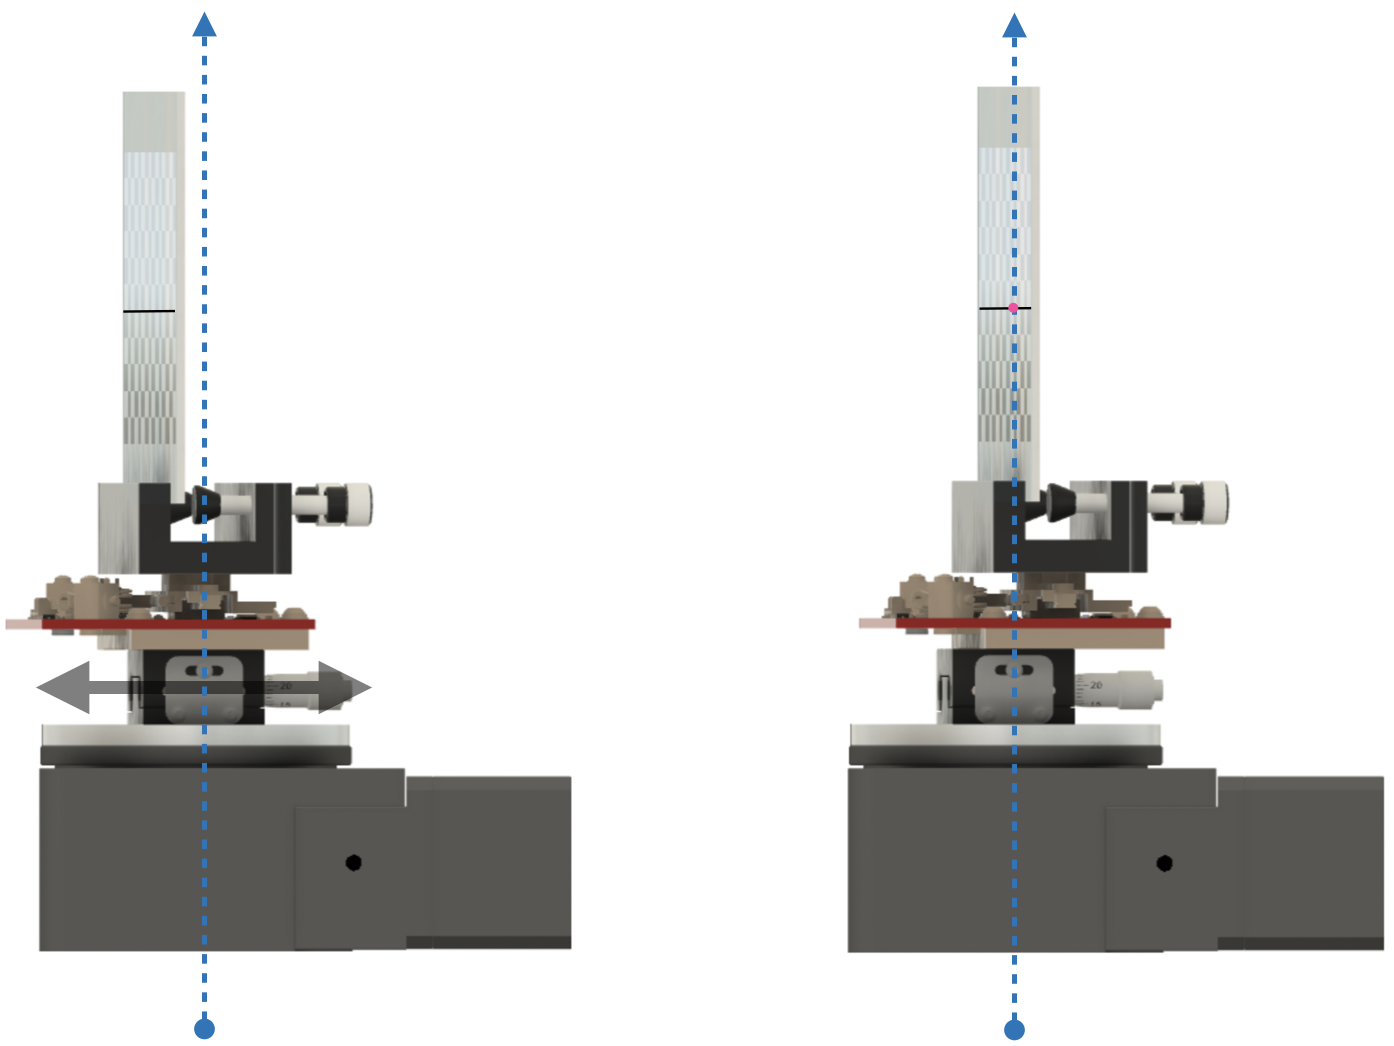
\includegraphics[width=0.5\linewidth]{figures/compact_alignment.png}
    \caption{Sample motion assembly without sample mount}
    \label{fig:compact_alignment}
\end{figure}

\section{Aligning Sample Motion Assembly and Illumination Beams} % alignBeams()
The objectives for beam alignment are to orient the two laser beams such that their intersection point is located on the RT-3 and RT-5 rotation axes, and their mean direction is perpendicular to the rotation axes. This ensures that that both beams' speckle images are generated from the same region in the sample and that the same region is sampled as we rotate the illuminators through the range of scattering angles.

Alignment proceeds as following. Given collinear azimuthal and RT-3 rotation axes, we can treat them as one axes with direction $\uvec{h}$ and location $\vec{P_h}$. This axis is located in the plane of a calibration target from previous alignment steps. For a beam spot a $\vec{Q}_{a_0} \in \mathbb{R}^3$ located on the plane, the displacement vector from the beam spot to the axis is $\vec{\Delta}_0 = \vec{P_h} + \vec{d}_0 - (\vec{P_h} + \uvec{h} \vec{d}_0^\intercal \uvec{h})$. We use a PID controller to displace the beam by $\vec{Delta}_0$ to within a tenth of the beam diameter. We repeat this for the second beam so both beam spots are located on the azimuthal axis. With beam spots a and b now located at $\vec{Q}_{a_1}, \vec{Q}_{b_1}$, we steer both beams to their mean position $\vecol{Q}$ so their intersection is located on the azimuthal axis.

\begin{figure}
    \centering
    \begin{subfigure}{0.49\textwidth}
        \centering
        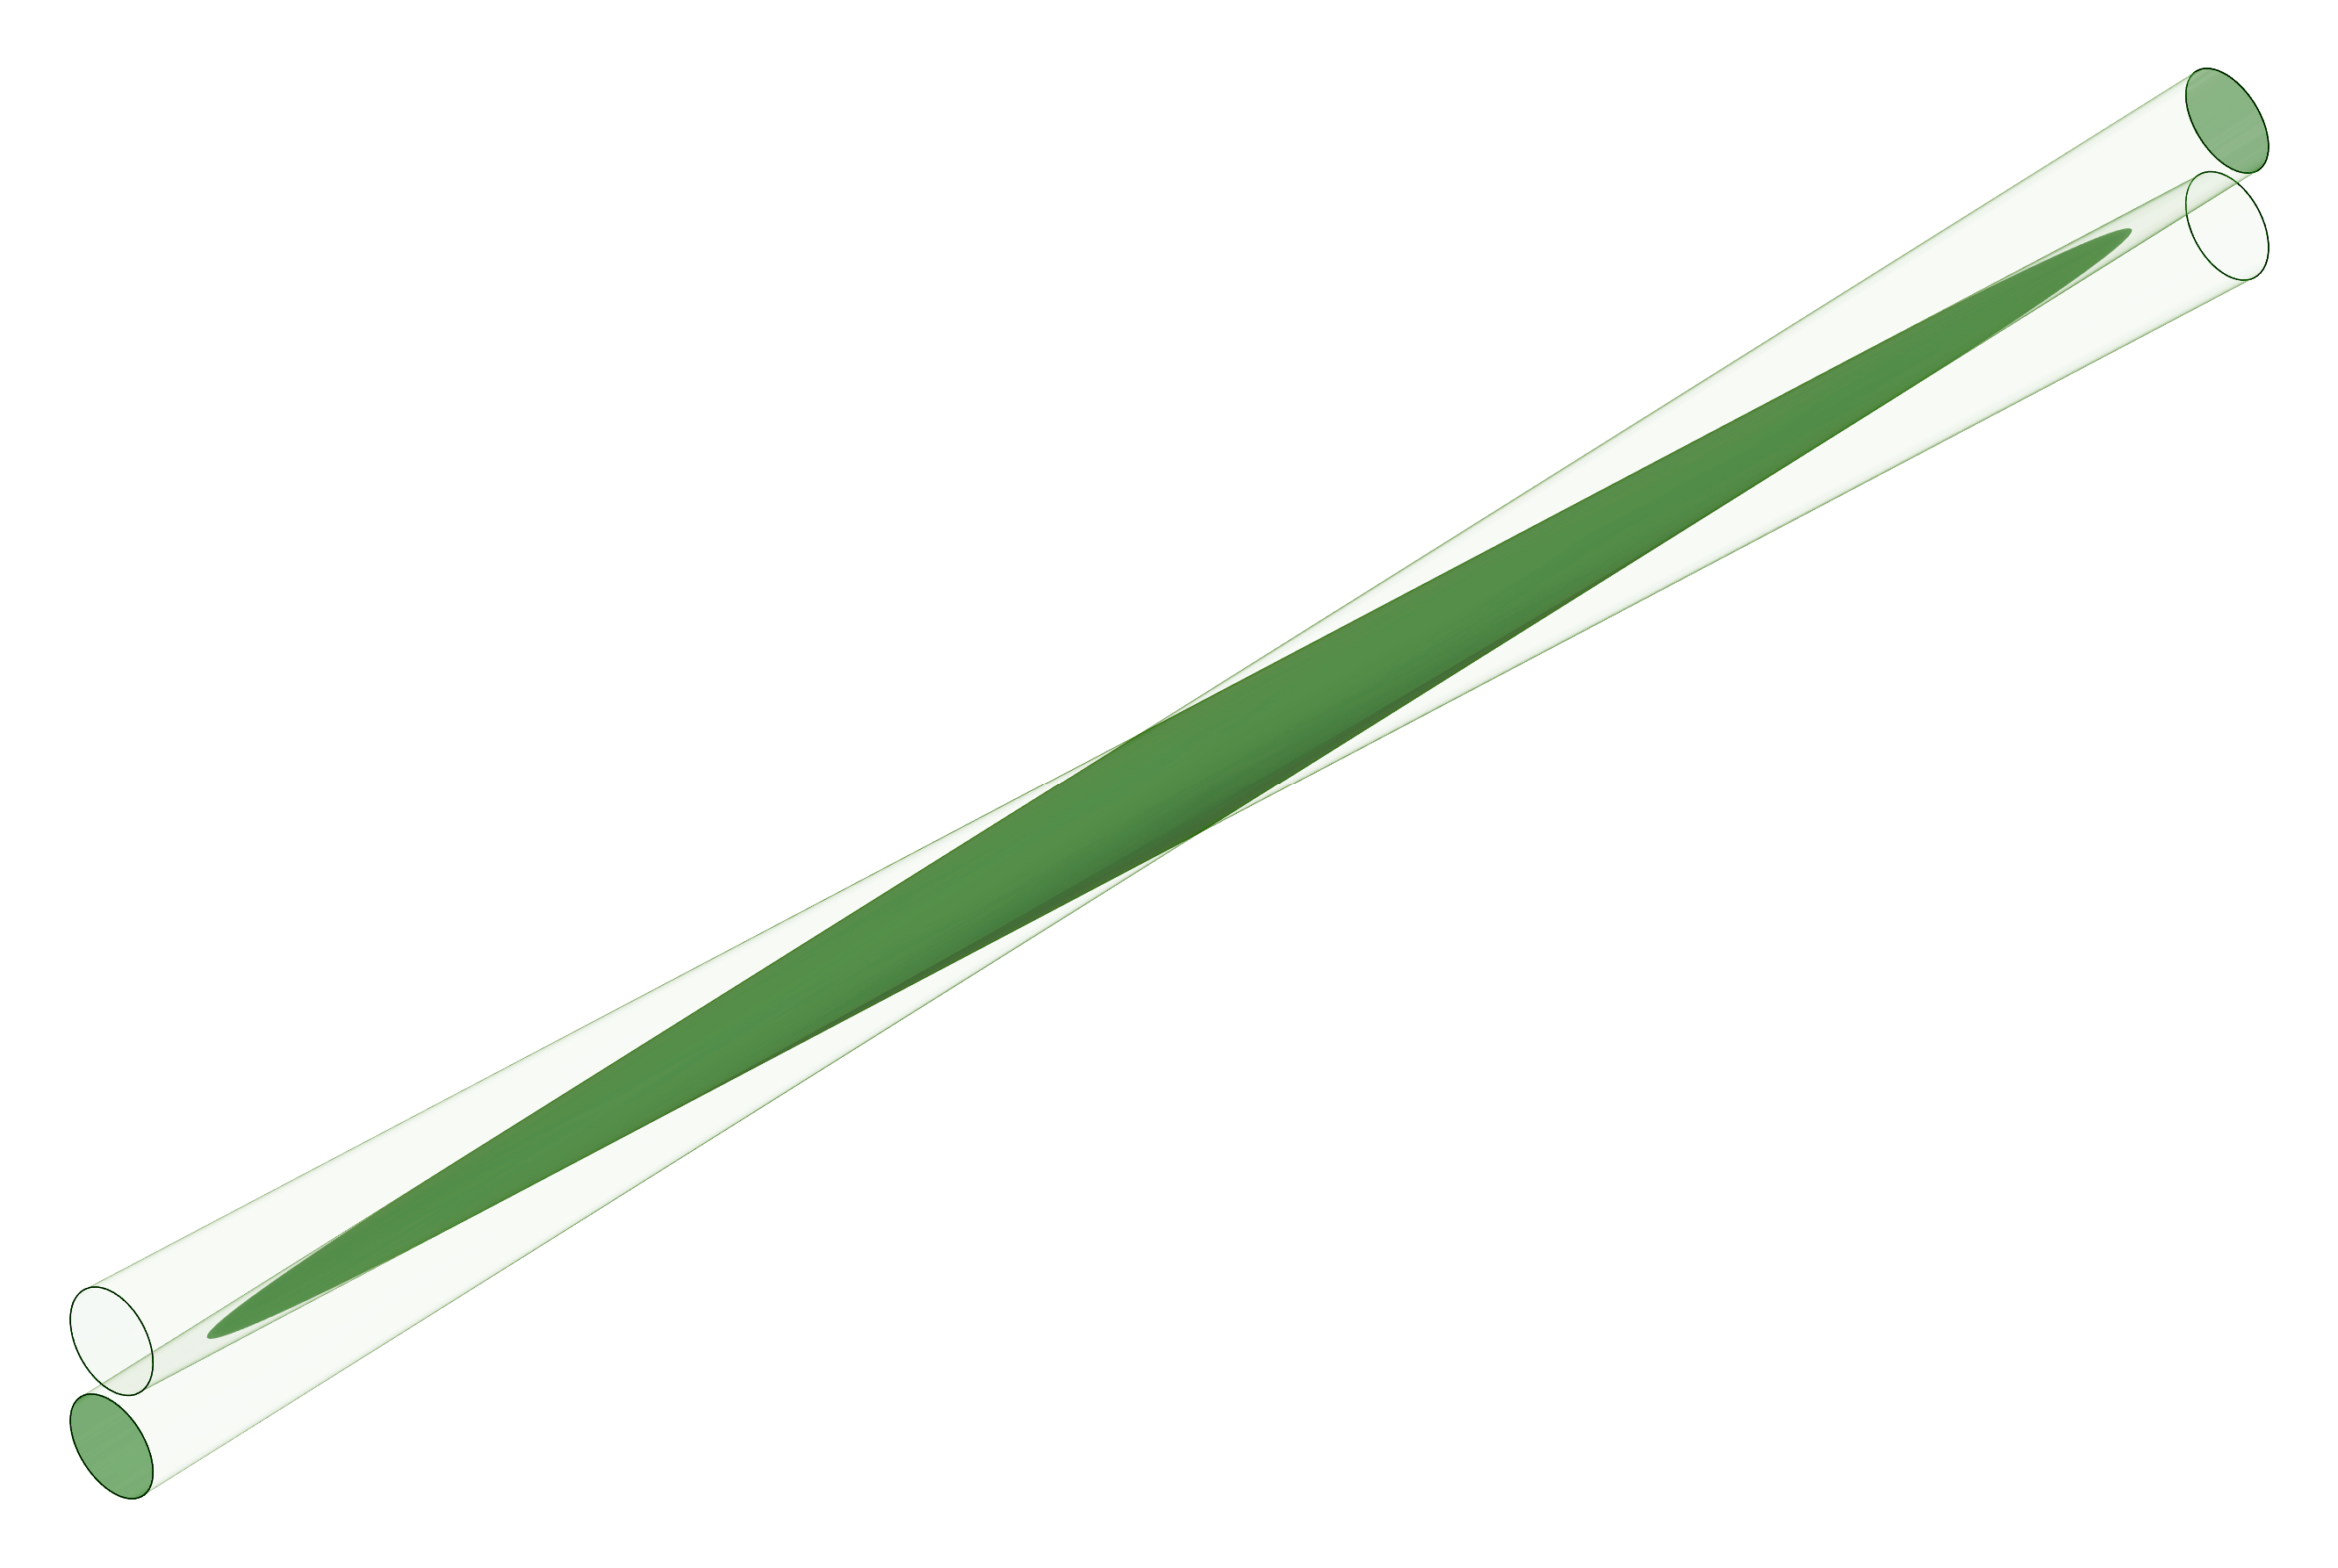
\includegraphics[width = \textwidth]{figures/beam_intersection_nooutline.png}
        \caption{Left figure}
        \label{fig:left}
    \end{subfigure}
    \begin{subfigure}{0.49\textwidth}
        \centering
        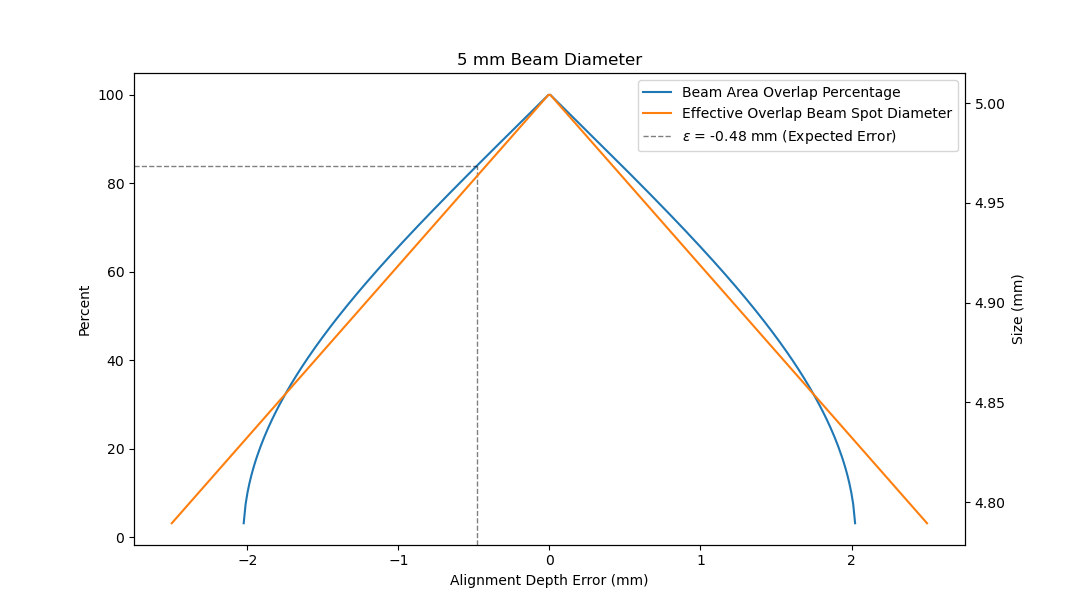
\includegraphics[width = \textwidth]{figures/BeamAlignmentMargin.png}
        \caption{Right figure}
        \label{fig:right}
    \end{subfigure}
    \caption{Combined figure}
    \label{fig:beam_intersection_margin}
\end{figure}

%
\begin{equation}
    \ell = 2 \frac{d_0}{\sin{\theta}} \cos{\theta/2}
\end{equation}
%
\begin{equation}
    d = 2 \frac{d_0}{\sin{\theta}} \sin{(\theta/2)}
\end{equation}

Both beams are equiangular with respect to the azimuthal axis when their projections onto the axis are equal and opposite.:
\begin{equation}
    0 = \uvec{k}_a^\intercal \vec{h} + \uvec{k}_b^\intercal \vec{h}.
    \label{eqn:beam_equiangular_objective}
\end{equation}

\begin{figure}
    \centering
    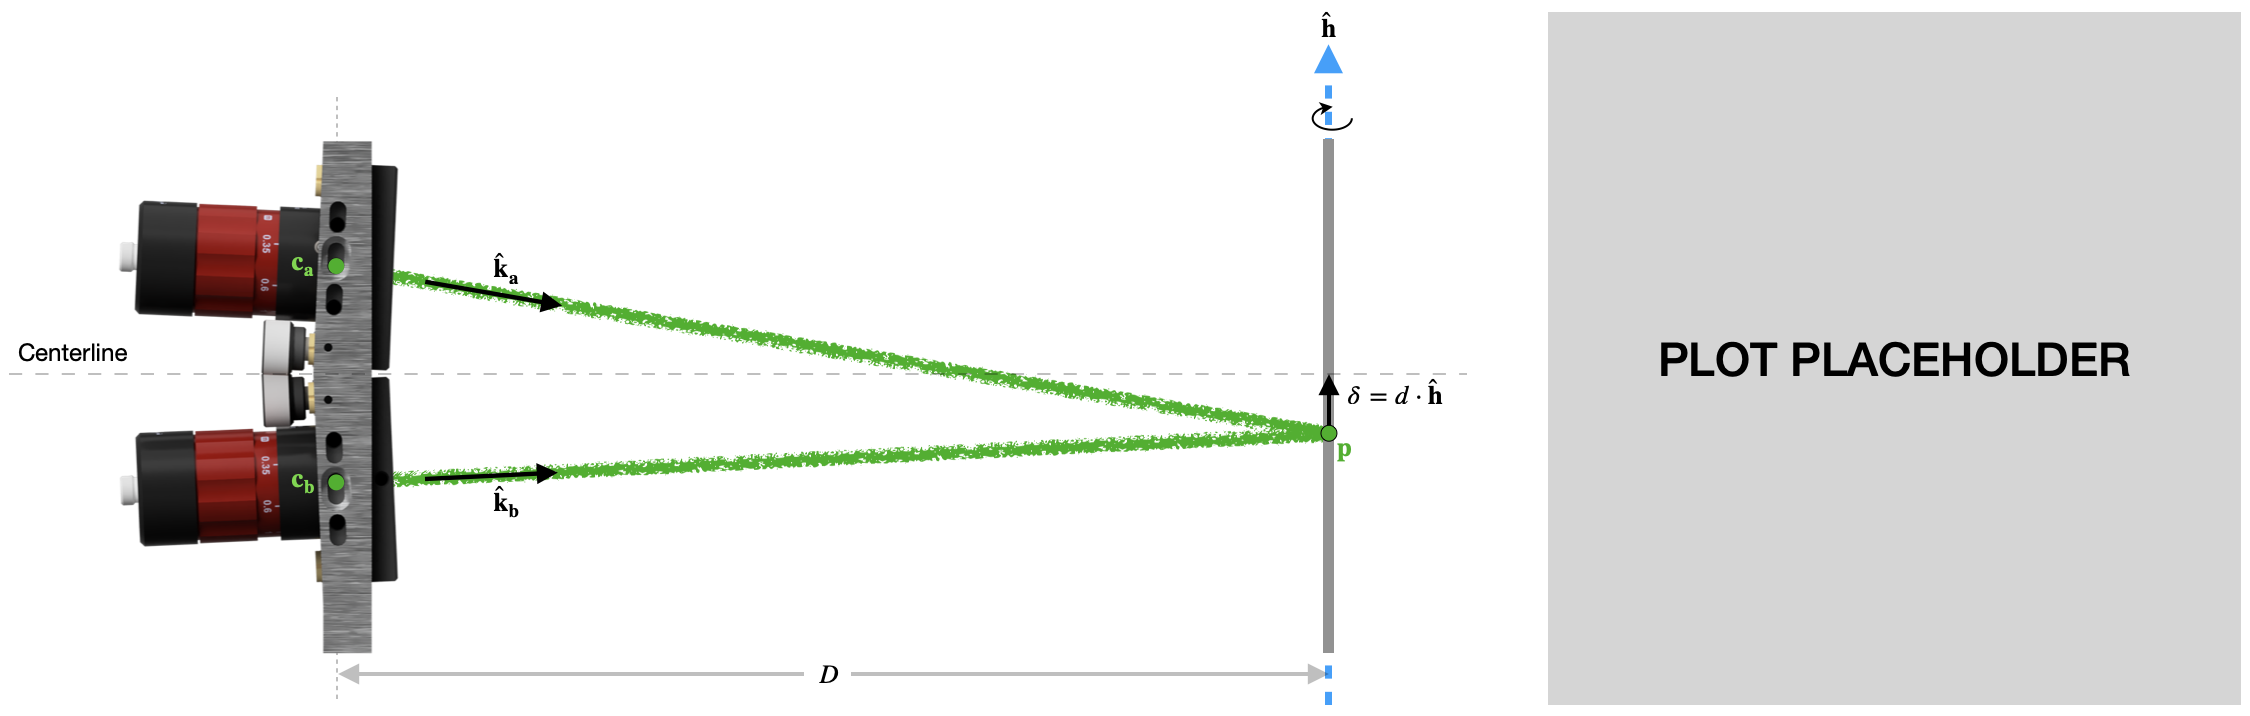
\includegraphics[width=\linewidth]{figures/beam_alignment_geometry.png}
    \caption{}
    \label{fig:beam_alignment_geometry}
\end{figure}
%
Define both beams' collimators positions $\vec{c}_a, \vec{c}_b$. The ideal intersection point $\vec{Q}^*$ is located at the intersection of the collimators' horizontal plane of symmetry and the azimuthal axis. $\vecol{Q}$ is offset from the ideal intersection point by displacement vector $\vec{\delta} = \vec{Q}^* - \vec{Q} = d \cdot \uvec{h}$. Equation \ref{eqn:beam_equiangular_objective} can be rewritten in terms of these variables to solve for the displacement distance $d$ along $\uvec{h}$:
\begin{equation}
    \begin{split}
    0 &= (\vec{Q} + \vec{\delta} - \vec{c_a})^\intercal \uvec{h} + (\vec{Q} + \vec{\delta} - \vec{c_b})^\intercal \vec{h} \\
    2 \vec{\delta}^\intercal \uvec{h} &= (\vec{c_a} - \vec{Q})^\intercal \uvec{h} + (\vec{c_b} - \vec{Qp})^\intercal \vec{h} \\
    2 \vec{\delta}^\intercal \uvec{h} &= (\vec{c_a} - \vec{Q} + \vec{c_b} - \vec{Q})^\intercal \uvec{h} \\
    d \cdot \uvec{h}^\intercal \uvec{h} &= \tfrac{1}{2} (\vec{c_a} - \vec{Q} + \vec{c_b} - \vec{Q})^\intercal \uvec{h} \\
    d &= \tfrac{1}{2} \big[(\vec{c_a} - \vec{Q}) + (\vec{c_b} - \vec{Q})\big]^\intercal \uvec{h}
    \end{split}
\end{equation}
%
The displacement vectors $\vec{c_a} - \vec{p}$ and $\vec{c_b} - \vec{Q}$ are unknown since the collimator positions are unknown. However, the normalized beam directions $\uvec{k}_a, \uvec{k}_b$ are parallel to these displacement vectors, so we approximate a scaling coefficient $s$ to achieve the correct scale. We determine $s$ using the CAD model based on the nominal design geometry, and the final beam intersection displacement expression is
%
\begin{equation}
    d = -\frac{s}{2} (\uvec{k}_a + \uvec{k}_b)^\intercal \uvec{h}.
    \label{eqn:beam_alignment_displacement}
\end{equation}

The alignment procedure is as follows. Since the beams' orientations have been adjusted since their initial estimation, we begin by updating their estimates. We use a method similar to that detailed in section \ref{sec:lower_stage_calibration}, but we use a single azimuthal position $\theta = 0$ rather than rotating the beam pair azimuthally. With update $\uvec{k}_a$ and $\uvec{k}_b$, and we compute the required intersection point displacement via Equation \ref{eqn:beam_alignment_displacement}. The displacement is projected into the image frame, and the beams are commanded to the corresponding pixel backprojected to the calibration target. This process is repeated iteratively until the displacement distance is below a threshold due to the approximate scale factor $s$ and other noise sources.

\section{Aligning Calibration Target with Illumination Beams}
This alignment step determines the "home" position of the sample assembly's rotation stage which corresponds to sample illumination along its normal vector. The home position maximizes the inner product of the target's normal vector and the mean illumination beam vector $\overline{\vec{k}} = (\uvec{k}_a + \uvec{k}_b)/2$.
\begin{figure}
    \centering
    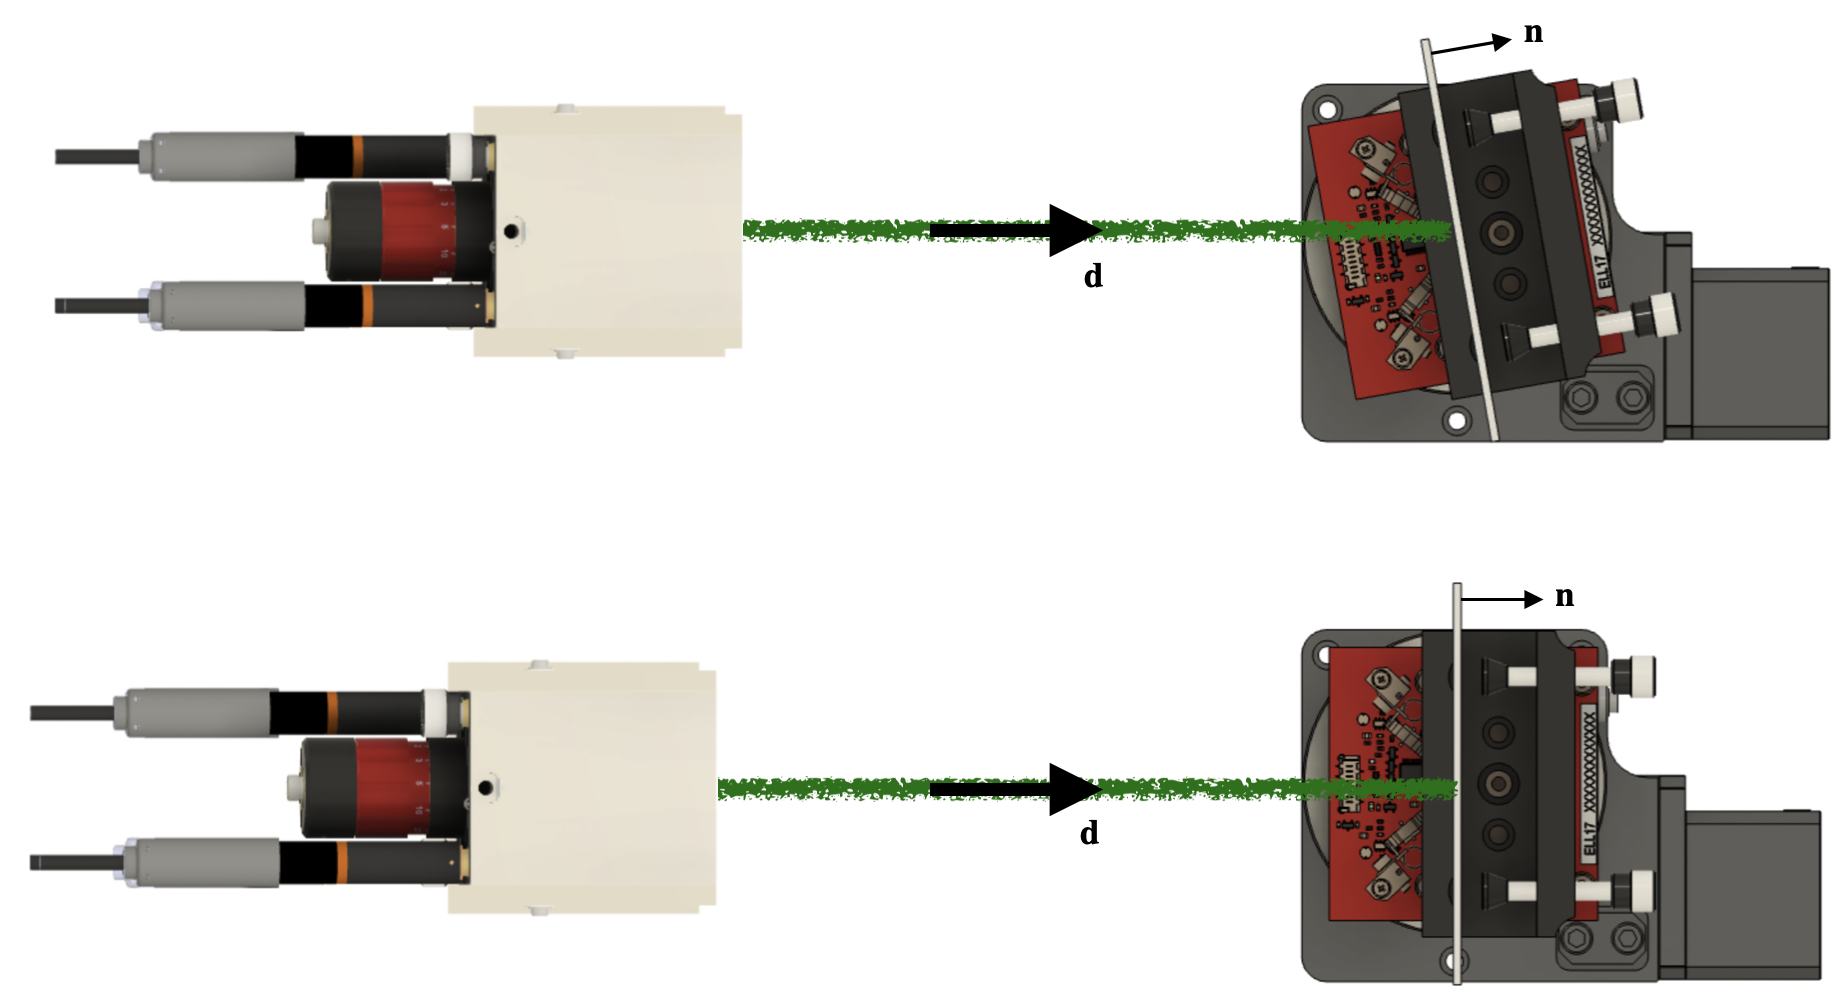
\includegraphics[width=0.5\linewidth]{figures/target_alignment.png}
    \caption{Top: Target and beam misaligned due to non-zero angle between the beam and the target normal; Bottom: $\vec{d}$ aligned with normal vector $\vec{n}$. \note{Update by replacing d with kbar.}}
    \label{fig:sample_beam_alignment}
\end{figure}

\section{\note{Proposal:}Acquisition Camera Calibration}
The projection matrix can be estimated via PnP in theory. However, we found it challenging in practice due to 3D points at infinity providing no depth information, and the geometry of a camera focused at infinity producing unstable estimates due to an effective coupling of the intrinsic parameters. \note{Add reasons they fail}. Since the acquisition camera maps points from the plane at infinity to the image plane, the homography for these planes is the projection matrix. However, there is an effective coupling of intrinsic parameters that complicates decomposing the projection matrix into a product of intrinsic and extrinsic matrices. 

A camera focused at infinity maps rays along its optical axis to its principal point; all directions measured relative to the optical axis are mapped to image points relative to the principal point. Translating the principal point is similar to rotating the camera externally under the small angle approximation $\tan(\phi) \approx \phi$. Therefore, these two parameters are effectively coupled for a non-WFOV camera. \note{Insert figure showing reprojection error loss vs. pp and rotation}. To avoid this issue, we estimate the focal length using a simple geometric relationship describing pinhole cameras focused at infinity followed principal point estimation via inspection. Once the intrinsics are known, we estimate the rotation matrix and the lens distortion coefficients simultaneously.

\subsection{Intrinsics}
Rays entering the camera at an angle $\phi$ with respect to the optical axis are mapped to a point $f_{px} \tan(\phi)$ pixels from the principal point. This relation can be used to estimate the focal length given a set of rays with known directions and their corresponding image pixel coordinates. Since beam directions are known for all azimuth angles from lower stage calibration \note{Insert reference}, we acquire images of beams rotated azimuthally, we compute the ray angle with respect to the optical axis and the pixel spacing. If we plot the pixel spacing vs. the tangent of the local ray angle, the line of best fit has a slope equal to the equivalent pinhole's focal length. We estimate the principal point by shining a collimated source into the lens oriented so it is approximately parallel to the lens' optical axis. The location of its image is assumed to be the principal point.
\begin{figure}
    \centering
    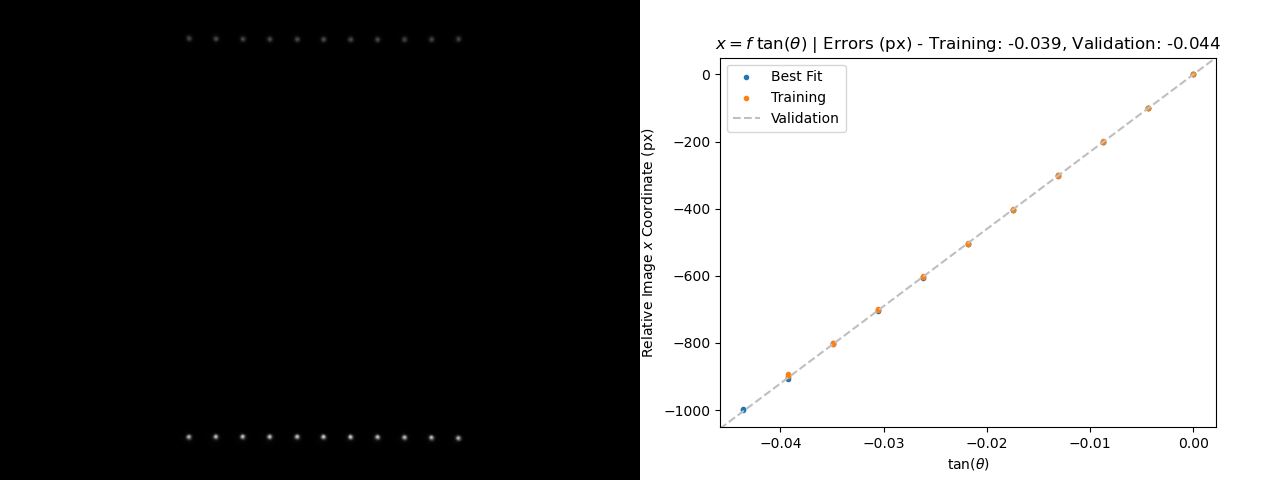
\includegraphics[width=0.75\linewidth]{figures/focal_length_estimate.png}
    \caption{Left: Composite of 11 images of both illuminators spanning an azimuth range $3.5^\circ$. Right: The acquisition camera's focal length is the constant of proportionality of image point displacement and the tangent of the internal ray angle with respect to the optical axis.}
    \label{fig:focal_length_estimate}
\end{figure}

\subsection{Extrinsics \& Lens Distortion}
\note{Newton-Raphson method via pytorch-minimize}.

\subsection{Validation}
The calibration model is validated on the physical acquisition system by learning a model on training data and then evaluating performance via a validation dataset. First, a checkerboard calibration target is placed at two different locations, and its poses are determined using a calibrated camera. A laser is attached to a rotation stage, and an image of the beam spot on the target is acquired at each position. The 3D beam-plane intersection point is then calculated using beam spot centroiding to find the pixel coordinates which are backprojected to the camera's frame using the camera matrix. The rotation stage axis $\mathbf{h}$ is determined by placing a target face-up on the stage and estimating the target's normal with the camera.


\paragraph{Validation Results} Figure \ref{fig:3}d shows the training and validation estimation errors of 3D points. Angles less than $90^\circ$ correspond to the target illuminated from the front with $0^\circ$ corresponding to Figure \ref{fig:3}c. Those to the right correspond to a back-illuminated target with $180^\circ$ being anti-normal. The training and validation errors have similar trends with reduced validation error, suggesting the data was not over-fit. There is no error benchmark rooted in a performance metric. However, since centroiding and the homography computed during calibration both have sub-pixel accuracy and this is ultimately an interpolation task, the targeted prediction accuracy is sub-pixel. Considering the minimum validation error is 1.5 pixels with a mean error of 2.8 pixels, the targeted accuracy seems achievable if the issue of worsening error with angle of incidence is alleviated and the beam direction estimates are improved.



\section{\note{Proposal:}Illuminator Assembly Calibration}
The goal for calibrating the illuminator assembly is estimating its rotation axis and the 3D orientation of the illumination beams as a function of the azimuth angle $\theta$. We do so by computing the 3D intersection of each illumination beam with a series of $N$ planes whose poses we know. This process is repeated for all $\theta \in \Theta$ for a total of $2N|\Theta|$ points. From this point set, we can estimate illumination directions for both beams as a function of $\theta$ and the azimuth stage pose up to a rotational ambiguity about its rotation axis.

\paragraph{\note{Proposal:}Azimuth Stage Rotation Axis}
Each beam is associated with a set of $N|\Theta|$ points. Define a set of difference vectors $\{\tilde{\vec{k}}_\theta\}, \; |\{\tilde{\vec{k}}_\theta\}| = L$ as the differences between all N permute 2 points along a ray. We define a ray as a beam located at any particular $\theta \in \Theta$. Each $\tilde{\vec{k}}_\theta$ makes an angle $\pi/2 - \alpha$ with the rotation axis. However, the $_L P_2$ 2nd order difference vectors are perpendicular to the azimuth rotation axis $\uvec{h}$, and we estimate $\uvec{h}$ as their null space.

\paragraph{\note{Proposal:}Beam Direction Vector}
Once we know the azimuth rotation axis, we can use it to estimate both illuminators' beam directions. For each $\theta \in \Theta$, we compute the centroid $\vecol{p}_\theta = \frac{1}{N} \sum p_n$. We subtract the centroid from the point set so it is zero mean, and we rotate it about $\uvec{h}$ by $-\theta$ so all points are aligned with $\theta = 0$. The beam direction $\vec{k}_0$ is simply the point set's principal component. For any arbitrary azimuthal angle $\theta$, we can compute the beam direction $\vec{k}_0 = \vec{R}_{\uvec{h}} \vec{k}_0$ where $\vec{R}_{\uvec{h}}$ is a $3 \times 3$ rotation matrix with azimuthal axis $\uvec{h}$.

\subsection{\note{Proposal:}Stage Position \& Beam Direction as a Function of $\theta$}
Assume a collimated beam fixed to a rotation stage with location $\vec{r}$ and rotation axis $\uvec{h}$. If the stage is rotated 360 degrees, the pencil of rays created by the rotated beam will form a paraboloid with axis $\uvec{h}$ and small radius $\rho$ equal to the distance of closest encounter of the beam with the paraboloid axis. The locus of these points of closest encounter constitute the beam's ray envelope. The isoline of the ray envelope is
%
\begin{figure}
    \centering
    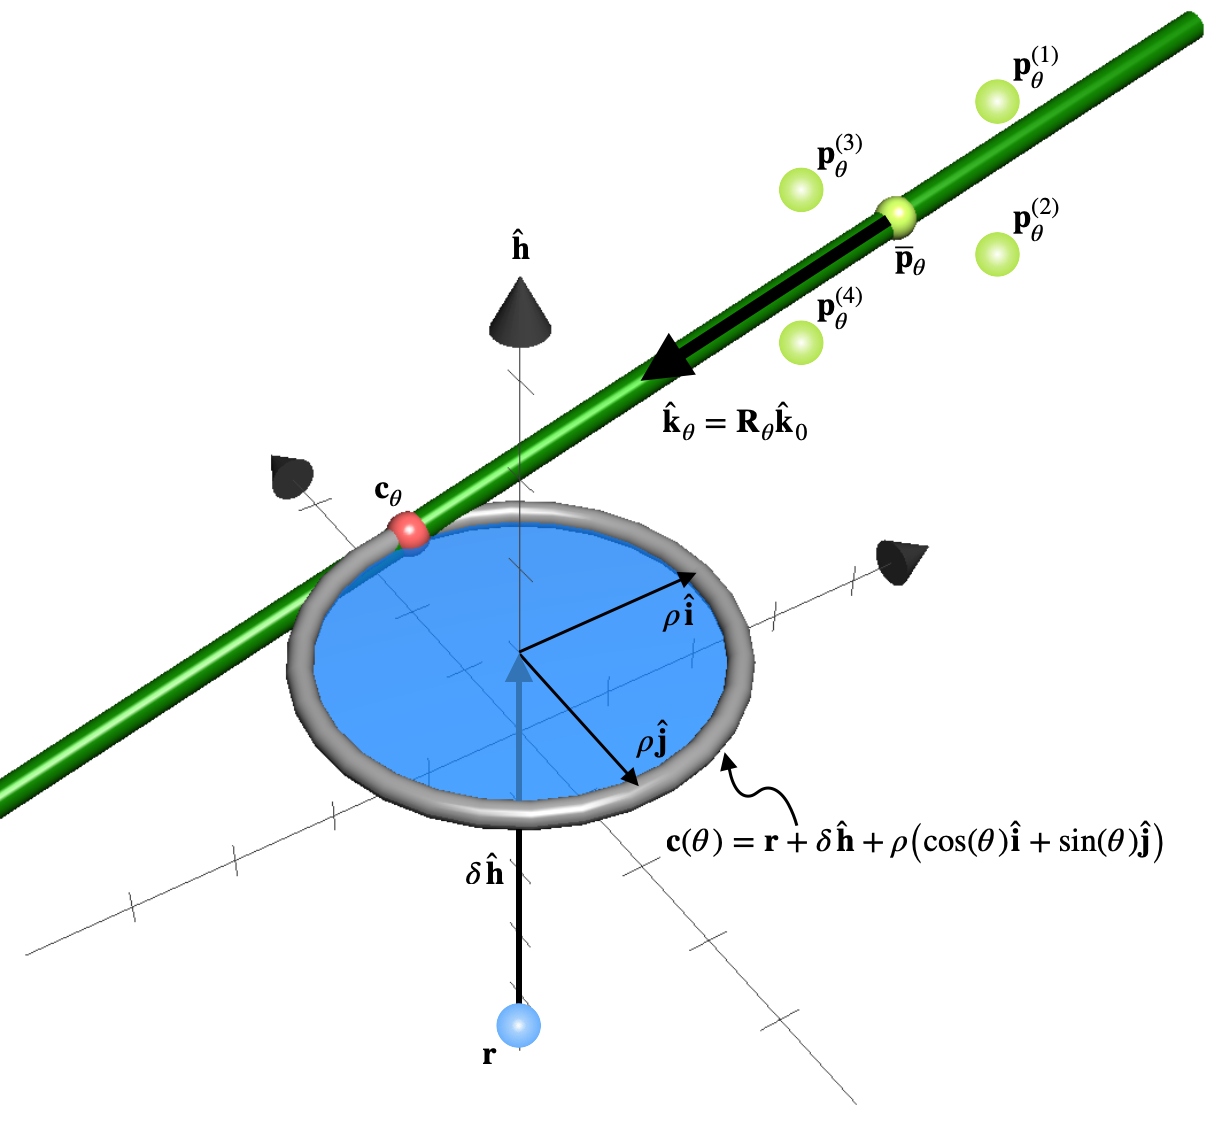
\includegraphics[width=0.5\linewidth]{figures/ray_envelope.png}
    \caption{Ray envelope defined as the locus of points of closest encounter between the illumination beam and its rotation axis}
    \label{fig:ray_envelope_geometry}
\end{figure}
%
\begin{equation}
    \vec{c}(\theta) = \vec{r} + \delta \uvec{h} + r(\theta) \vec{\rho}_0,
    \label{eqn:envelope2}
\end{equation}
%
where $\delta$ is the height of the circle above the stage, $\vec{\rho}$ is a $2 \times 1$ vector. $r(\theta)$ is a $3 \times 2$ matrix consisting of a rotation of two basis vectors $\uvec{i}$ and $\uvec{j}$ through an angle of $\theta$ about the rotation axis $\uvec{h}$ with each basis vector being perpendicular to $\uvec{h}$
%
\begin{equation}
    r(\theta) = \vec{R}(\uvec{h}, \theta) \begin{bmatrix}
        \uvec{i} & \uvec{j}
    \end{bmatrix},
    \quad \vec{R}(\uvec{h}, \theta) \in \mathbb{R}^{3 \times 3}.
\end{equation}

If $M$ points $\vec{p}_\theta^{(1)}, \vec{p}_\theta^{(2)}, ..., \vec{p}_\theta^{(M)}$ are measured along the ray at a given rotation stage position $\theta \in \Theta$, then the beam with direction $\uvec{k}_{\theta}$ passes through their centroid $\vecol{p}_\theta$ with its pencil defined
%
\begin{align}
    \vec{l}_\theta(s) = \vecol{p}_\theta + s \uvec{k}_{\theta}
\end{align}

\section{Acquisition Camera Calibration}
The projection matrix can be estimated using PnP in theory. However, we found it challenging in practice due to 3-D points at infinity providing no depth information, resulting in unstable estimation. Since the acquisition camera maps points from the plane at infinity to the image plane, the homography relating these planes is the projection matrix. However, there is an effective coupling of intrinsic and extrinsic parameters that complicates decomposing the projection matrix into a product of intrinsic and extrinsic matrices.

A camera focused at infinity maps rays parallel to its optical axis to its principal point; all directions measured relative to the optical axis are mapped to image points relative to the principal point. If $p$ is the distance of a pixel from the principal point of a camera with focal length $f$, then $p = f \tan(\phi)$ for an incoming ray at angle $\theta$ with respect to the optical axis. Under the small angle approximation, $p \approx f\phi$ which means the pixel distance change proportionally to the incoming ray angle. Therefore, shifting the principal point is analogous to rotating the camera externally for small angles, and these two parameters are effectively coupled for a non-WFOV camera. This numerical coupling results in a reprojection error loss topology that is not strictly convex as shown in Figure \ref{fig:acquisition_camera_calibration}(c). Therefore, we estimate the intrinsics by computing the focal length as the ambiguity's constant of proportionality and choosing a principal point. Once the intrinsics are known, we estimate the rotation matrix and the lens distortion coefficients simultaneously.

Since the focal length is the constant of proportionality for beam angle and image pixel displacement and the beam directions are known for all azimuth angles from illuminator assembly calibration, we can compute the focal length. We acquire images of the two illumination beams rotated azimuthally and compute ray angles with respect to the optical axis. If we plot the pixel spacing vs. the tangent of the local ray angle, the line of best fit has a slope equal to the equivalent pinhole camera's focal length (Figure \ref{fig:acquisition_camera_calibration}(a,b). We separately estimate the principal point by shining a collimated source into the lens oriented so it is approximately parallel to the lens' optical axis. The location of its image is assumed to be the principal point. Finally, we estimate the camera's rotation matrix and lens distortion coefficients numerically as the parameters that minimize the reprojection error given the previously determined focal length and principal point.
\begin{figure}
    \centering
    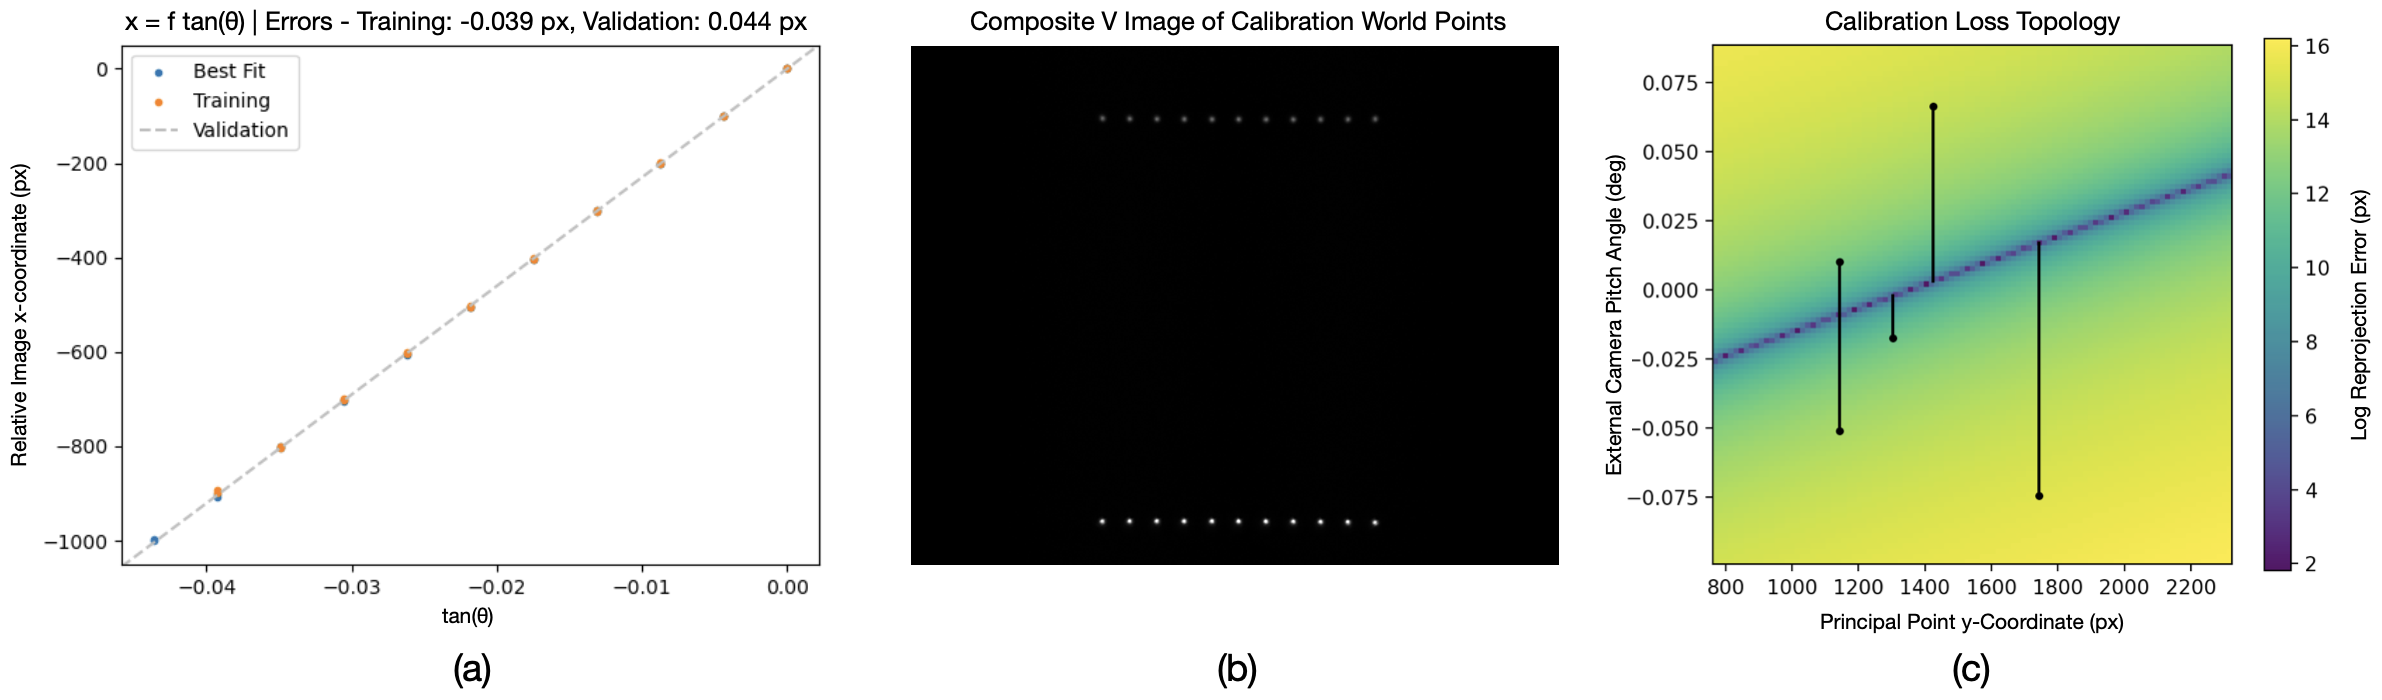
\includegraphics[width=\linewidth]{figures/acqusition_camera_calibration.png}
    \caption{(a) The acquisition camera's focal length is the constant of proportionality of image point displacement and the tangent of the internal ray angle with respect to the optical axis; (b) Composite of 11 images of both illuminators spanning an azimuth range $3.5^\circ$; (c) Reprojection error as a function of principal point shifts along the y-axis and external pitch rotation is not strictly convex, showing the numerical ambiguity of principal point shifting and camera rotation. This ambiguity holds for the x-axis and panning as well.}
    \label{fig:acquisition_camera_calibration}
\end{figure}


\section{\note{Proposal:}Acquisition Light Efficiency}
Given a linearly polarized illumination laser beam, an acquisition sensor offset by a scattering angle $\theta$, and a scattering sample inside a glass cell, the goal is to determine 1) the optimal sample orientation and 2) the optimal angle of polarization to maximize light transmitted from the illuminator to the acquisition sensor. All theory below assumes scattering particles are small compared with the wavelength and are detailed in \cite{born2013principles}.

\subsubsection{\note{Proposal:}Fresnel Formulae}
Consider a plane wave with amplitude A incident on a surface. The electric and magnetic field vectors can be decomposed into two components parallel and perpendicular to the surface plane. The incident electric field is
%
\begin{equation}
    E^{(i)} = 
    \begin{bmatrix}
        -A_{||} \cos{\theta_i} e^{-i \tau_i} \\
        A_\perp e^{-i \tau_i} \\
        A_{||} \sin{\theta_i} e^{-i \tau_i}
    \end{bmatrix}
\end{equation}
%
where $E_x, E_z$ are in the plane, $E_y$ is along the plane normal, and the complex exponential argument is defined
%
\begin{equation}
    \tau_i = \omega \big( t - \tfrac{\mathbf{r}^\intercal \mathbf{s^{(i)}}}{v} \big) = \omega \big( t - \tfrac{x \sin{\theta_i} + z \cos{\theta_i}}{v} \big).
\end{equation}

The magnetic field vector $H$ is written similarly through the relation $H = \sqrt{\epsilon} \mathbf{s} \times \mathbf{E}$.
where $\mathbf{s}$ is the light's velocity vector. If $T$ and $R$ denote the transmitted and reflected amplitudes, then the transmitted field is
%
\begin{equation}
    E^{(t)} = 
    \begin{bmatrix}
        -T_{||} \cos{\theta_t} e^{-i \tau_t} \\
        T_\perp e^{-i \tau_t} \\
        T_{||} \sin{\theta_t} e^{-i \tau_t}
    \end{bmatrix},
\end{equation}
%
and the reflected field is
%
\begin{equation}
    E^{(r)} = 
    \begin{bmatrix}
        -R_{||} \cos{\theta_r} e^{-i \tau_r} \\
        R_\perp e^{-i \tau_r} \\
        R_{||} \sin{\theta_r} e^{-i \tau_r}
    \end{bmatrix}.
\end{equation}

The tangential components of the electric and magnetic fields must be continuous across the boundary, resulting in four boundary conditions:
%
\begin{align}
    E^{(i)}_x + E^{(r)}_x = E^{(t)}_x \quad & E^{(i)}_y + E^{(r)}_y = E^{(t)}_y \\
    H^{(i)}_x + H^{(r)}_x = H^{(t)}_x \quad & H^{(i)}_y + H^{(r)}_y = H^{(t)}_y.
\end{align}

These boundary conditions can be solved for an expression of the transmitted and reflected amplitudes components by using the Maxwell relation $n = \sqrt{\epsilon}$
%
\begin{align}
    T_{||} = \frac{2 n_1 \cos{\theta_i}}{n_2 \cos{\theta_i} + n_1 \cos{\theta_t}} A_{||} \quad &
    T_{\perp} = \frac{2 n_1 \cos{\theta_i}}{n_1 \cos{\theta_i} + n_2 \cos{\theta_t}} A_{\perp} \\
    R_{||} = \frac{n_2 \cos{\theta_i} - n_1 \cos{\theta_t}}{n_2 \cos{\theta_i} + n_1 \cos{\theta_t}} A_{||} \quad &
    R_{\perp} = \frac{n_1 \cos{\theta_i} - n_2 \cos{\theta_t}}{n_1 \cos{\theta_i} + n_2 \cos{\theta_t}} A_{\perp}.
\end{align}

\subsubsection{\note{Proposal:}Effects of Polarization on Fresnel Formulae}

The light intensity is
%
\begin{equation}
    S = \frac{c}{4\pi} \sqrt{\epsilon} E^2 = \frac{cn}{4\pi} E^2
\end{equation}
%
The resulting energy incident on a surface with unit area $A$ is
%
\begin{equation}
    J^{(i)} = S^{(i)} \cos{\theta_i} = \frac{cn_1}{4\pi} |A|^2 \cos{\theta_i}
\end{equation}
%
with reflected and transmitted energies
%
\begin{align}
    J^{(r)} = \frac{cn_1}{4\pi} |R|^2 \cos{\theta_i} & \quad and \quad J^{(t)} = \frac{cn_2}{4\pi} |T|^2 \cos{\theta_t}.
\end{align}
%
The reflectivity and transmissivity are
%
\begin{align}
    \mathcal{R} = \frac{J^{(r)}}{J^{(i)}} = \frac{|R|^2}{|A|^2} & \quad and \quad \mathcal{T} = \frac{J^{(t)}}{J^{(i)}} = \frac{|T|^2}{|A|^2}
\end{align}
%
which satisfy the law of conservation of energy by summing to 1
%
\begin{equation}
    \mathcal{R} + \mathcal{T} = 1.
\end{equation}

The reflectivity and transmissivity are functions of polarization with respect to the parallel and perpendicular directions. If the incident electric field $\mathbf{E}$ makes an angle $\alpha_i$ with respect to the plane, the parallel and perpendicular area components are
%
\begin{align}
    A_{||} = A \cos{\alpha_i} & \quad and \quad A_{\perp} = A \sin{\alpha_i}
\end{align}
%
The parallel energy component of the incident light is
%
\begin{align}
    J_{||}^{(i)} &= \frac{cn_1}{4\pi} |A_{||}|^2 \cos{\theta_i} \nonumber \\
    &= \frac{cn_1}{4\pi} |A |^2 \cos^2{\alpha_i} \cos{\theta_i} \nonumber \\
    &= J^{(i)} \cos^2{\alpha_i}
\end{align}
%
with that of the perpendicular component following similarly:
%
\begin{equation}
    J_{\perp}^{(i)} = J^{(i)} \sin^2{\alpha_i}.
\end{equation}
%
The reflectivity in terms of polarized light is
%
\begin{align}
    \mathcal{R} = \frac{J^{(r)}}{J^{(i)}} &= \frac{J_{||}^{(r)} + J_{\perp}^{(r)}}{J^{(i)}} \nonumber \\
    &= \frac{J_{||}^{(r)}}{J_{||}^{(i)}} \cos^2{\alpha_i} + \frac{J_{\perp}^{(r)}}{J_{\perp}^{(i)}} \sin^2{\alpha_i} \nonumber \\
    &= \mathcal{R}_{||} \cos^2{\alpha_i} + \mathcal{R}_{\perp} \sin^2{\alpha_i},
\end{align}
%
and the transmissivity is
%
\begin{equation}
    \mathcal{T} = \mathcal{T}_{||} \cos^2{\alpha_i} + \mathcal{T}_{\perp} \sin^2{\alpha_i}.
\end{equation}
%
Reflectivity and transmissivity must satisfy conservation of energy respectively:
%
\begin{equation}
    \mathcal{R}_{||} + \mathcal{T}_{||} = 1, \qquad \mathcal{R}_{\perp} + \mathcal{T}_{\perp} = 1.
\end{equation}

When light is incident normal to the surface, $\alpha_i = 0$ for all E-field orientations, meaning there is no distinction between the parallel and perpendicular components, and the reflectivity and transmissivity are written
%
\begin{equation}
    \mathcal{R} = \bigg(\frac{n - 1}{n+1} \bigg)^2, \qquad \mathcal{T} = \frac{4n}{(n + 1)^2}
\end{equation}
%
where $n = n_2 / n_1$.

% \subsubsection{Fresnel Relations as Mueller Matrices}
% \paragraph{Transmission Mueller Matrix}
% %
% \begin{equation}
%     \Mv_t = \frac{9|a_1|^2}{4k^2r^2}
%     \begin{bmatrix}
%         \tfrac{1}{2}(t_s^2 + t_p^2) & \tfrac{1}{2}(t_s^2 - t_p^2) & 0 & 0 \\
%         \tfrac{1}{2}(t_s^2 - t_p^2) & \tfrac{1}{2}(t_s^2 + t_p^2) & 0 & 0 \\
%         0 & 0 & t_s t_p & 0 \\ 
%         0 & 0 & 0 & t_s t_p
%     \end{bmatrix}
% \end{equation}

% \paragraph{Scattering Mueller Matrix}
% Assuming light with wavevector $k$ is scattered from a small sphere with radius $a$ with scattering amplitude coefficient $a_1 \in \mathbb{C}$, the scattered field at distance $r$ from the scatterer, the Mueller matrix is
% %
% \begin{equation}
%     \Mv_s = \frac{9|a_1|^2}{4k^2r^2}
%     \begin{bmatrix}
%         \tfrac{1}{2}(1 + \cos^2{\theta}) & \tfrac{1}{2}(\cos^2{\theta} - 1) & 0 & 0 \\
%         \tfrac{1}{2}(\cos^2{\theta} - 1) & \tfrac{1}{2}(1 + \cos^2{\theta}) & 0 & 0 \\
%         0 & 0 & \cos{\theta} & 0 \\ 
%         0 & 0 & 0 & \cos{\theta}
%     \end{bmatrix}
% \end{equation}
% %
% where the scattering coefficient is defined
% %
% \begin{equation}
%     a_1 = -\frac{i2x^3}{e} \frac{m^2 - 1}{m^2 + 2} - \frac{i2x^5}{5} \frac{(m^2 - 2)(m^2 - 1)}{(m^2 + 2)^2}
% \end{equation}
% %
% with scale factor and relative refractive index
% %
% \begin{equation}
%     x = ka = \frac{2 \pi N a}{\lambda},  \qquad m = \frac{N_1}{N} = \frac{k_1}{k}
% \end{equation}
% %
% where $N$ and $N_1$ are the medium's and particle's refractive indices respectively \cite{bohren2008absorption}. The scattering Mueller matrix is defined within the scattering plane containing the incoming and outgoing directions as well as the scattering particle.

These relations were used to find the optimal sample assembly rotation angle and the angle of polarization for every acquisition scattering angle. The result is a lookup table plotted as a chart in Figure \ref{fig:polctrl}.
%
\begin{figure}
    \centering
    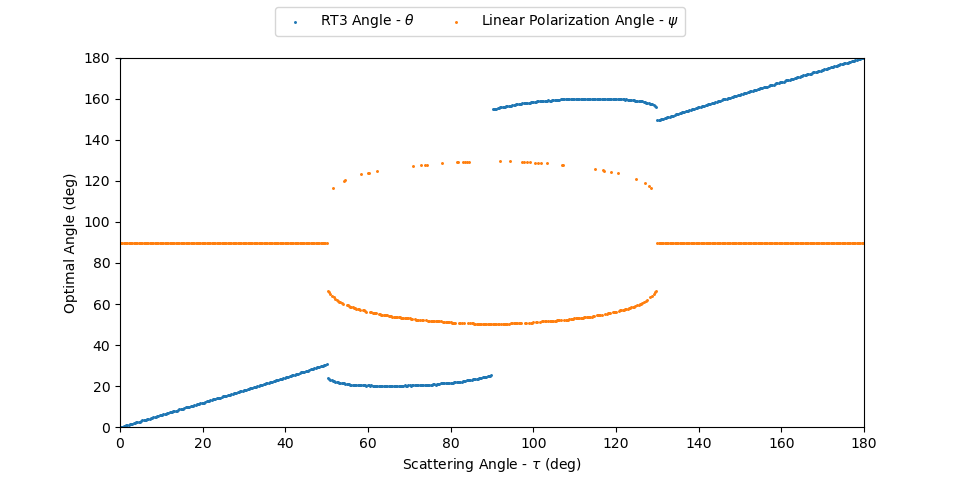
\includegraphics[width=0.49\linewidth]{figures/polctrl1_traj.png}
    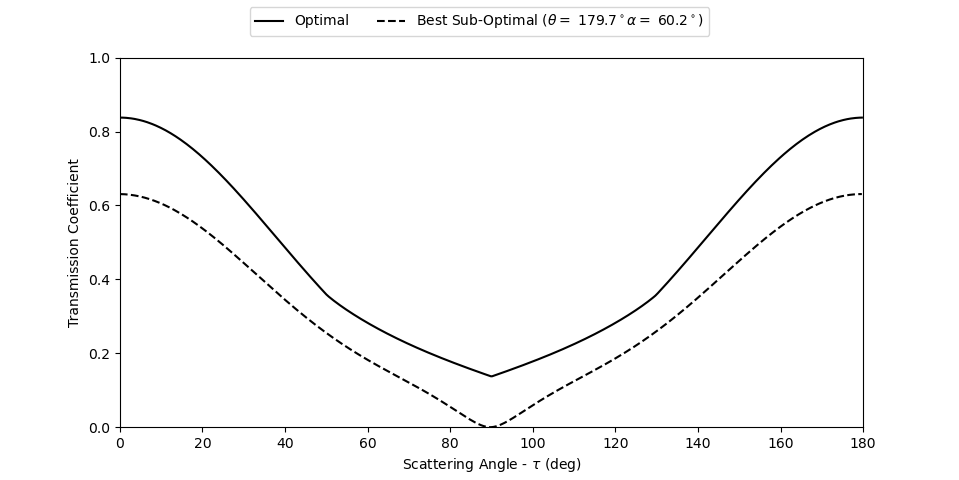
\includegraphics[width=0.49\linewidth]{figures/polctrl1_trans.png}
    \caption{Left: Optimal sample rotation stage position and linear polarization angle as a function of azimuthal illumination angle. The linear polarization angle schedule contains discontinuities in the range $(-50^\circ, 50^\circ)$ due to rounding errors; Right: Comparison of light transmitted towards camera when choosing the optimal sample orientation versus a static sample shows an approximate 15\% increase on average.}
    \label{fig:polctrl}
\end{figure}

\section{\note{Proposal:}Expected Results}
We have identified imaging configurations that produce high-contrast speckle images with well-resolved speckle grains through HDR acquisition and proper camera specifications. Examples of images we have acquired to date are shown in Figure \ref{fig:speckle_collage}. These speckle images are high-contrast which is indicative of a suitable beamwidth (5mm) for the sample's scattering cross-section, and the speckle grains are well-resolved, meaning the camera's angular resolution is sufficient.
%
\begin{figure}
    \centering
    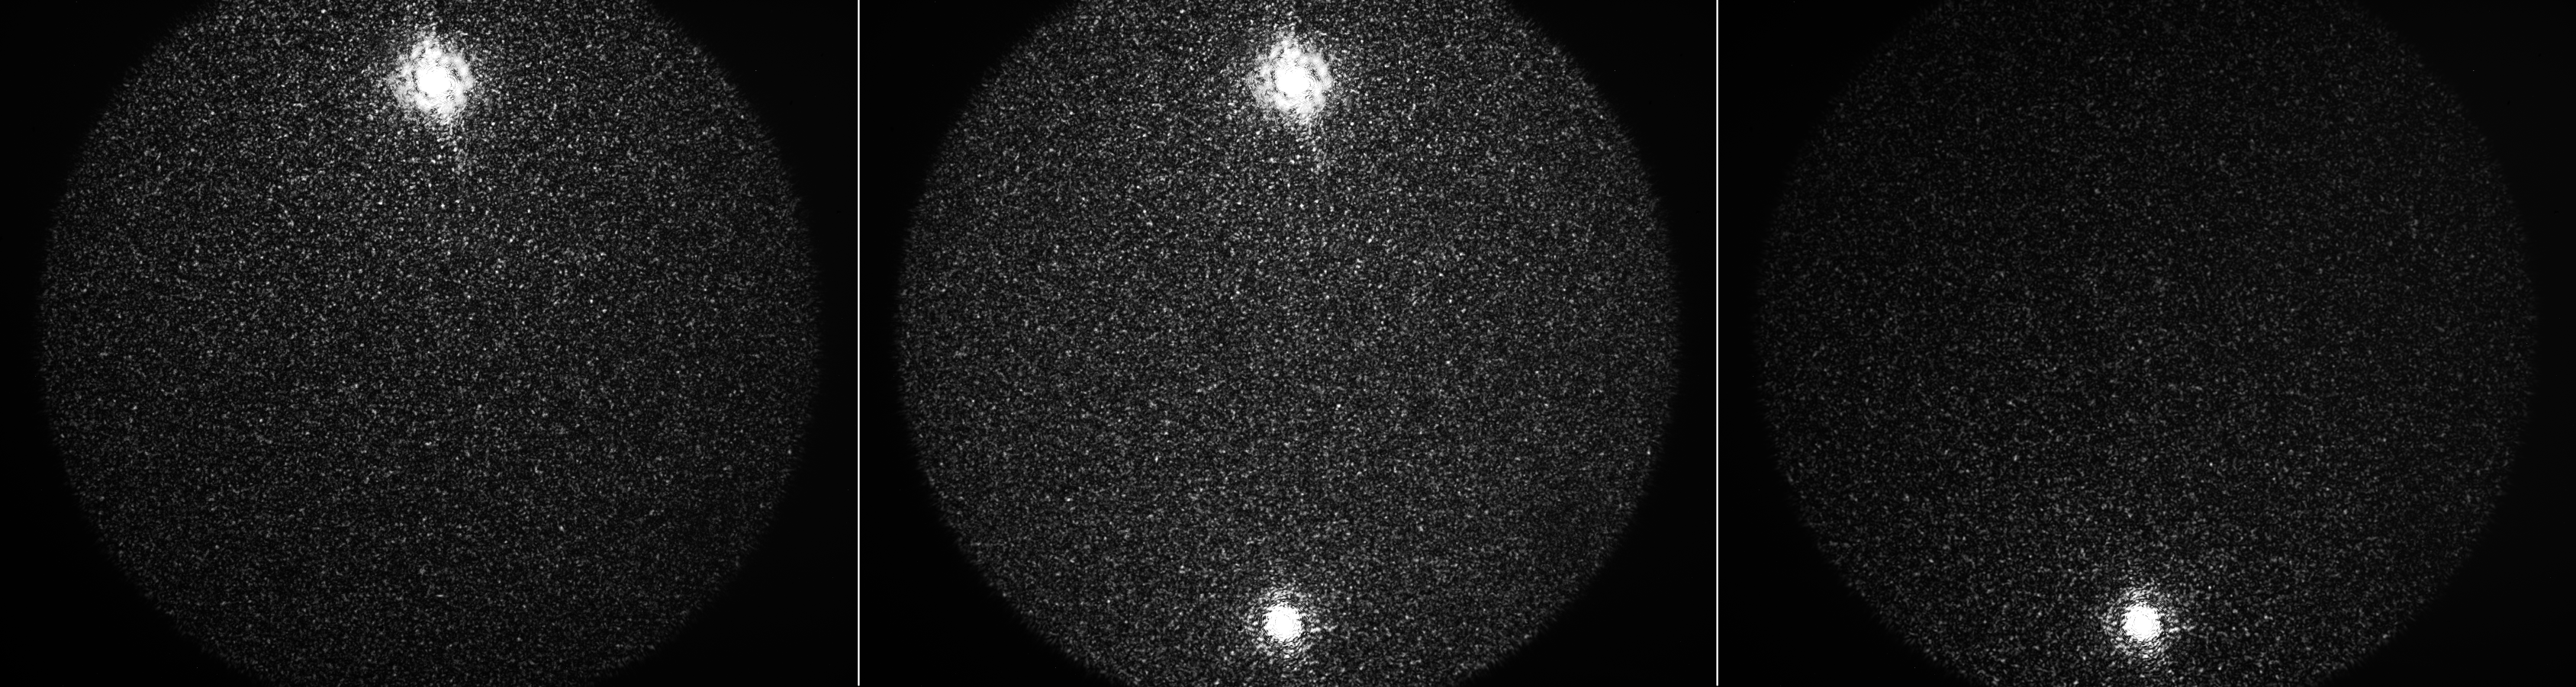
\includegraphics[width=\textwidth]{figures/speckle_collage.png}
    \caption{Speckle images of 10$\mu$m monodisperse SiO$_2$ beads acquired using scatterometer setup. Left: Top illuminator activated; Center: Both illuminators activated; Right: Bottom illuminator activated}
    \label{fig:speckle_collage}
\end{figure}

A preliminary result that indicates we are on the right track is computing and plotting 2D speckle correlation and showing that this correlation increases with decreasing sample optical density. Next, we plan to acquire phase functions of materials similar those acquired in \cite{alterman2022direct} over a larger range of scattering angles. Figure \ref{fig:extended_phase_function} shows our planned extension of the scattering angle range. If our phase functions agree with \cite{alterman2022direct}, it will help validate our acquisition configuration and correlation scripts.
%
\begin{figure}
    \centering
    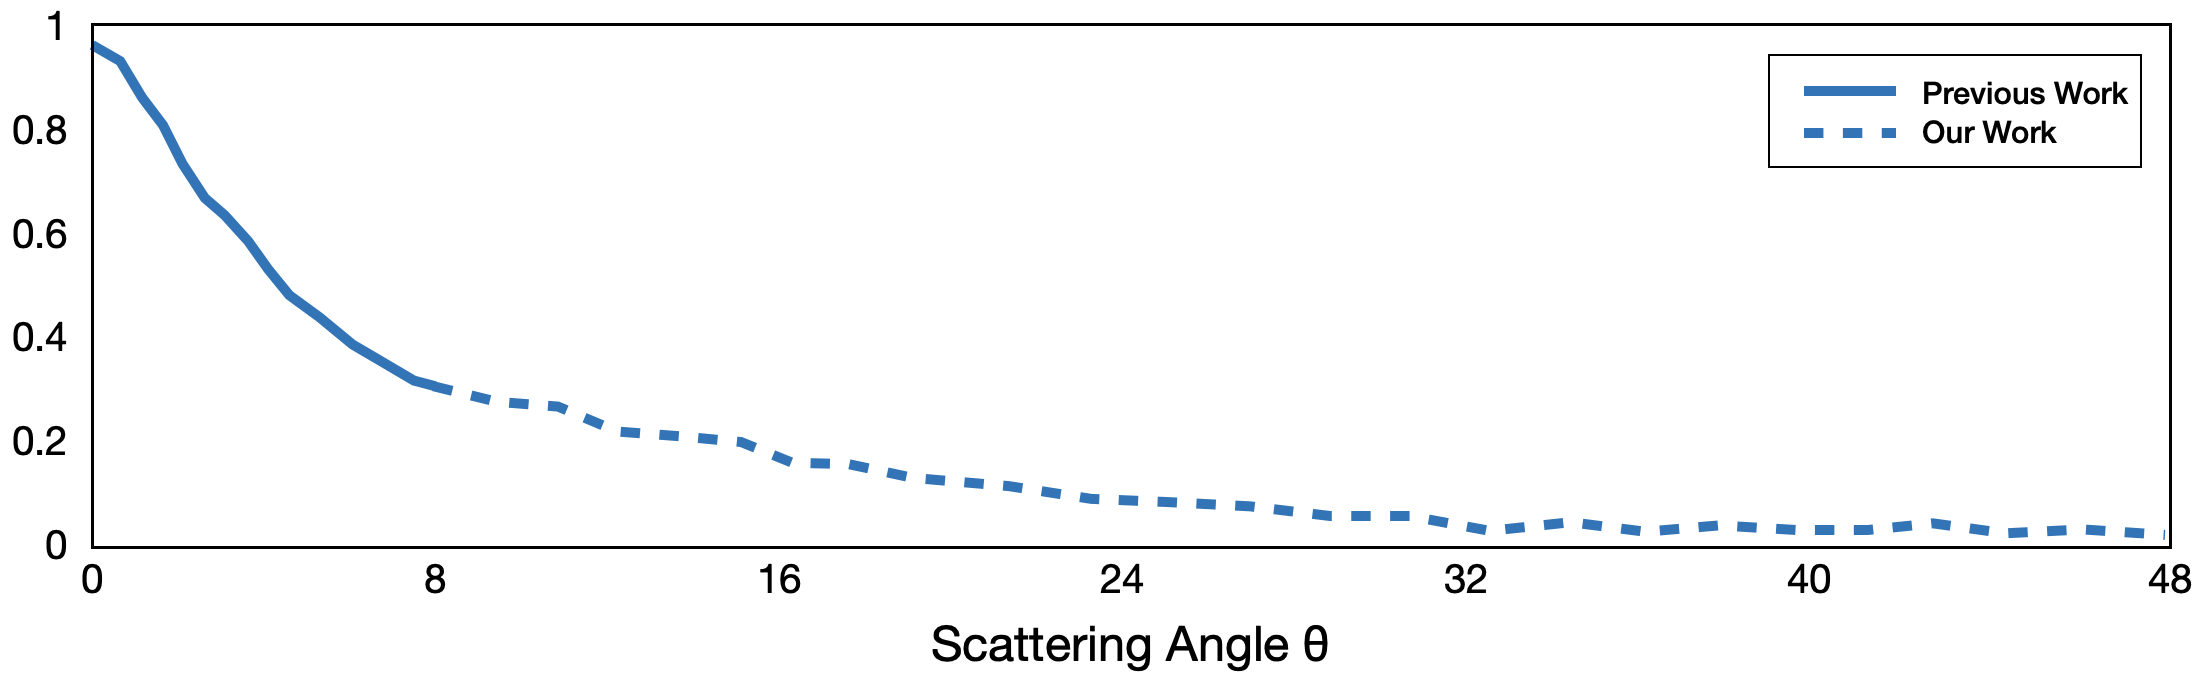
\includegraphics[width=\textwidth]{figures/extended_phase_function.png}
    \caption{An expected result is acquiring the scattering phase function for a larger range of scattering angles than the literature.}
    \label{fig:extended_phase_function}
\end{figure}